% ================================================================
% The printable version of latex/starters/targeted/KS3/fractions/introductoryFractionsStarters.tex
%
% This is the same deck, laid out to be handed out rather than put on
% the board. Every slide is shown as it stands before any answer is
% revealed, and 4 copies of it go on one page of A4, two by two, so
% that a printed page cuts into four question sheets.
%
%   made from           latex/starters/targeted/KS3/fractions/introductoryFractionsStarters.tex
%   slides on the sheet 9
%   copies of each      4, two by two on A4 landscape
%   printing rules      version 2
%
% Nothing was reworded and nothing was rewritten. Each slide is the slide
% from the deck, asked for at its first step, which is how the answers
% stay hidden.
%
% Please don't edit this file. It is written again from the one it was
% made from whenever that changes, so an edit here would be lost - edit
% that file instead and this one follows.
% ================================================================
\documentclass{beamer}
\usepackage{tikz}
\usetikzlibrary{calc}
\usepackage{xcolor}
\usepackage{multicol}

% ================================================================
% Answer-overlay helpers
% ================================================================
\newcommand{\ablank}[1]{%
  \alt<2>{\textcolor{red}{#1}}{\underline{\phantom{#1}}}%
}
\newcommand{\ashow}[1]{\uncover<2->{\textcolor{red}{\small #1}}}
\newcommand{\ashowq}[1]{\alt<2->{\textcolor{red}{\small #1}}{?}}

% Answers drawn straight on to a TikZ diagram, revealed on overlay 2 like \ashow.
% Space is reserved on overlay 1, so the diagram does not move between slides.
\usetikzlibrary{overlay-beamer-styles}
\tikzset{
  ans/.style     = {red, thick, visible on=<2->},
  ansfill/.style = {red!15, visible on=<2->},
  anslab/.style  = {red, font=\tiny, visible on=<2->},
}

\title{Fractions: Starters}
\author{}
\date{}

% ---------------------------------------------------------------
% Added so this deck prints four slides to a page. Nothing above
% this line was changed.
% ---------------------------------------------------------------
\usepackage{pgfpages}

% 4 slides to a sheet of A4, two by two, with a thin line round each
% so that the page can be cut up.
%
% Each slide keeps a margin of 1mm around it and no more, so the four fill
% the sheet and the pieces they cut into are as big as the paper allows. Only
% one direction actually comes out that tight: a slide is a different shape
% from a quarter of a sheet of A4, so it is scaled to fit and the slack it
% cannot use is left along whichever pair of edges it did not fill.
\pgfpagesuselayout{4 on 1}[a4paper,landscape,border shrink=1mm]
\pgfpageslogicalpageoptions{1}{border code=\pgfusepath{stroke}}
\pgfpageslogicalpageoptions{2}{border code=\pgfusepath{stroke}}
\pgfpageslogicalpageoptions{3}{border code=\pgfusepath{stroke}}
\pgfpageslogicalpageoptions{4}{border code=\pgfusepath{stroke}}

% There is nothing on paper to click, and a slide announcing a new section
% would sit between two copies of the same question and put every page after
% it out of step with the grid.
\setbeamertemplate{navigation symbols}{}
\AtBeginPart{}
\AtBeginSection{}
\AtBeginSubsection{}
\AtBeginSubsubsection{}
\begin{document}

\frame{\titlepage}

%------------------------------------------------
% SLIDE 1: Equal Sharing and Part-Whole (Merged)
%------------------------------------------------
\begin{frame}<1>{Starter 1}

\begin{columns}
\column{0.45\textwidth}
\begin{center}
\begin{tikzpicture}[scale=0.85]
% A: Unequal
\draw (0,0) rectangle (1.2,1.2);
\draw (0,0.4) -- (1.2,0.4);
\draw (0.3,0) -- (0.3,1.2);
\fill[blue!20] (0,0) rectangle (0.3,0.4);
\node at (0.6,-0.3) {A};
% B: Equal
\draw (2,0) rectangle (3.2,1.2);
\draw (2,0.6) -- (3.2,0.6);
\draw (2.6,0) -- (2.6,1.2);
\fill[blue!20] (2,0) rectangle (2.6,0.6);
\node at (2.6,-0.3) {B};
% C: Equal
\draw (0,-1.8) circle (0.7);
\draw (0,-1.8) -- (0.7,-1.8);
\draw (0,-1.8) -- (-0.7,-1.8);
\draw (0,-1.8) -- (0,-1.1);
\draw (0,-1.8) -- (0,-2.5);
\fill[green!20] (0,-1.8) -- (0.7,-1.8) arc (0:90:0.7) -- cycle;
\node at (0,-2.8) {C};
% D: Unequal
\draw (2,-1.8) circle (0.7);
\draw (2,-1.8) -- (2.7,-1.8);
\draw (2,-1.8) -- (2,-1.1);
\draw (2,-1.8) -- (1.3,-1.8);
\fill[green!20] (2,-1.8) -- (2,-1.1) arc (90:180:0.7) -- cycle;
\node at (2,-2.8) {D};

% --- Q3 answer: a rectangle in 5 equal parts, 3 of them shaded ---
\fill[ansfill, red!35] (0,-4.4) rectangle (1.8,-3.8);
\draw[ans] (0,-4.4) rectangle (3,-3.8);
\foreach \x in {0.6,1.2,1.8,2.4} \draw[ans] (\x,-4.4) -- (\x,-3.8);
\node[anslab, below] at (1.5,-4.45) {Q3: $\tfrac{3}{5}$};
\end{tikzpicture}
\end{center}

\column{0.55\textwidth}
\textbf{Questions}
\begin{enumerate}
    \item Which shapes (A, B, C, D) are divided into equal parts? \ashow{B and C}
    \item In shape B, what fraction is shaded? \ashow{$\frac{1}{4}$}
    \item Draw a rectangle divided into 5 equal parts. Shade $\frac{3}{5}$.
    \item Which is larger: $\frac{2}{5}$ or $\frac{3}{5}$? \ashow{$\frac{3}{5}$}
    \item Which is larger: $\frac{3}{5}$ or $\frac{3}{4}$? \ashow{$\frac{3}{4}$}
    \item Order the following fractions from smallest to largest: \newline $\frac{1}{100}, \frac{100}{1}, \frac{1}{10}, \frac{10}{1}, \frac{1}{1}$ \ashow{$\frac{1}{100},\ \frac{1}{10},\ \frac{1}{1},\ \frac{10}{1},\ \frac{100}{1}$}
\end{enumerate}
\end{columns}

\end{frame}
\begin{frame}<1>{Starter 1}

\begin{columns}
\column{0.45\textwidth}
\begin{center}
\begin{tikzpicture}[scale=0.85]
% A: Unequal
\draw (0,0) rectangle (1.2,1.2);
\draw (0,0.4) -- (1.2,0.4);
\draw (0.3,0) -- (0.3,1.2);
\fill[blue!20] (0,0) rectangle (0.3,0.4);
\node at (0.6,-0.3) {A};
% B: Equal
\draw (2,0) rectangle (3.2,1.2);
\draw (2,0.6) -- (3.2,0.6);
\draw (2.6,0) -- (2.6,1.2);
\fill[blue!20] (2,0) rectangle (2.6,0.6);
\node at (2.6,-0.3) {B};
% C: Equal
\draw (0,-1.8) circle (0.7);
\draw (0,-1.8) -- (0.7,-1.8);
\draw (0,-1.8) -- (-0.7,-1.8);
\draw (0,-1.8) -- (0,-1.1);
\draw (0,-1.8) -- (0,-2.5);
\fill[green!20] (0,-1.8) -- (0.7,-1.8) arc (0:90:0.7) -- cycle;
\node at (0,-2.8) {C};
% D: Unequal
\draw (2,-1.8) circle (0.7);
\draw (2,-1.8) -- (2.7,-1.8);
\draw (2,-1.8) -- (2,-1.1);
\draw (2,-1.8) -- (1.3,-1.8);
\fill[green!20] (2,-1.8) -- (2,-1.1) arc (90:180:0.7) -- cycle;
\node at (2,-2.8) {D};

% --- Q3 answer: a rectangle in 5 equal parts, 3 of them shaded ---
\fill[ansfill, red!35] (0,-4.4) rectangle (1.8,-3.8);
\draw[ans] (0,-4.4) rectangle (3,-3.8);
\foreach \x in {0.6,1.2,1.8,2.4} \draw[ans] (\x,-4.4) -- (\x,-3.8);
\node[anslab, below] at (1.5,-4.45) {Q3: $\tfrac{3}{5}$};
\end{tikzpicture}
\end{center}

\column{0.55\textwidth}
\textbf{Questions}
\begin{enumerate}
    \item Which shapes (A, B, C, D) are divided into equal parts? \ashow{B and C}
    \item In shape B, what fraction is shaded? \ashow{$\frac{1}{4}$}
    \item Draw a rectangle divided into 5 equal parts. Shade $\frac{3}{5}$.
    \item Which is larger: $\frac{2}{5}$ or $\frac{3}{5}$? \ashow{$\frac{3}{5}$}
    \item Which is larger: $\frac{3}{5}$ or $\frac{3}{4}$? \ashow{$\frac{3}{4}$}
    \item Order the following fractions from smallest to largest: \newline $\frac{1}{100}, \frac{100}{1}, \frac{1}{10}, \frac{10}{1}, \frac{1}{1}$ \ashow{$\frac{1}{100},\ \frac{1}{10},\ \frac{1}{1},\ \frac{10}{1},\ \frac{100}{1}$}
\end{enumerate}
\end{columns}

\end{frame}
\begin{frame}<1>{Starter 1}

\begin{columns}
\column{0.45\textwidth}
\begin{center}
\begin{tikzpicture}[scale=0.85]
% A: Unequal
\draw (0,0) rectangle (1.2,1.2);
\draw (0,0.4) -- (1.2,0.4);
\draw (0.3,0) -- (0.3,1.2);
\fill[blue!20] (0,0) rectangle (0.3,0.4);
\node at (0.6,-0.3) {A};
% B: Equal
\draw (2,0) rectangle (3.2,1.2);
\draw (2,0.6) -- (3.2,0.6);
\draw (2.6,0) -- (2.6,1.2);
\fill[blue!20] (2,0) rectangle (2.6,0.6);
\node at (2.6,-0.3) {B};
% C: Equal
\draw (0,-1.8) circle (0.7);
\draw (0,-1.8) -- (0.7,-1.8);
\draw (0,-1.8) -- (-0.7,-1.8);
\draw (0,-1.8) -- (0,-1.1);
\draw (0,-1.8) -- (0,-2.5);
\fill[green!20] (0,-1.8) -- (0.7,-1.8) arc (0:90:0.7) -- cycle;
\node at (0,-2.8) {C};
% D: Unequal
\draw (2,-1.8) circle (0.7);
\draw (2,-1.8) -- (2.7,-1.8);
\draw (2,-1.8) -- (2,-1.1);
\draw (2,-1.8) -- (1.3,-1.8);
\fill[green!20] (2,-1.8) -- (2,-1.1) arc (90:180:0.7) -- cycle;
\node at (2,-2.8) {D};

% --- Q3 answer: a rectangle in 5 equal parts, 3 of them shaded ---
\fill[ansfill, red!35] (0,-4.4) rectangle (1.8,-3.8);
\draw[ans] (0,-4.4) rectangle (3,-3.8);
\foreach \x in {0.6,1.2,1.8,2.4} \draw[ans] (\x,-4.4) -- (\x,-3.8);
\node[anslab, below] at (1.5,-4.45) {Q3: $\tfrac{3}{5}$};
\end{tikzpicture}
\end{center}

\column{0.55\textwidth}
\textbf{Questions}
\begin{enumerate}
    \item Which shapes (A, B, C, D) are divided into equal parts? \ashow{B and C}
    \item In shape B, what fraction is shaded? \ashow{$\frac{1}{4}$}
    \item Draw a rectangle divided into 5 equal parts. Shade $\frac{3}{5}$.
    \item Which is larger: $\frac{2}{5}$ or $\frac{3}{5}$? \ashow{$\frac{3}{5}$}
    \item Which is larger: $\frac{3}{5}$ or $\frac{3}{4}$? \ashow{$\frac{3}{4}$}
    \item Order the following fractions from smallest to largest: \newline $\frac{1}{100}, \frac{100}{1}, \frac{1}{10}, \frac{10}{1}, \frac{1}{1}$ \ashow{$\frac{1}{100},\ \frac{1}{10},\ \frac{1}{1},\ \frac{10}{1},\ \frac{100}{1}$}
\end{enumerate}
\end{columns}

\end{frame}
\begin{frame}<1>{Starter 1}

\begin{columns}
\column{0.45\textwidth}
\begin{center}
\begin{tikzpicture}[scale=0.85]
% A: Unequal
\draw (0,0) rectangle (1.2,1.2);
\draw (0,0.4) -- (1.2,0.4);
\draw (0.3,0) -- (0.3,1.2);
\fill[blue!20] (0,0) rectangle (0.3,0.4);
\node at (0.6,-0.3) {A};
% B: Equal
\draw (2,0) rectangle (3.2,1.2);
\draw (2,0.6) -- (3.2,0.6);
\draw (2.6,0) -- (2.6,1.2);
\fill[blue!20] (2,0) rectangle (2.6,0.6);
\node at (2.6,-0.3) {B};
% C: Equal
\draw (0,-1.8) circle (0.7);
\draw (0,-1.8) -- (0.7,-1.8);
\draw (0,-1.8) -- (-0.7,-1.8);
\draw (0,-1.8) -- (0,-1.1);
\draw (0,-1.8) -- (0,-2.5);
\fill[green!20] (0,-1.8) -- (0.7,-1.8) arc (0:90:0.7) -- cycle;
\node at (0,-2.8) {C};
% D: Unequal
\draw (2,-1.8) circle (0.7);
\draw (2,-1.8) -- (2.7,-1.8);
\draw (2,-1.8) -- (2,-1.1);
\draw (2,-1.8) -- (1.3,-1.8);
\fill[green!20] (2,-1.8) -- (2,-1.1) arc (90:180:0.7) -- cycle;
\node at (2,-2.8) {D};

% --- Q3 answer: a rectangle in 5 equal parts, 3 of them shaded ---
\fill[ansfill, red!35] (0,-4.4) rectangle (1.8,-3.8);
\draw[ans] (0,-4.4) rectangle (3,-3.8);
\foreach \x in {0.6,1.2,1.8,2.4} \draw[ans] (\x,-4.4) -- (\x,-3.8);
\node[anslab, below] at (1.5,-4.45) {Q3: $\tfrac{3}{5}$};
\end{tikzpicture}
\end{center}

\column{0.55\textwidth}
\textbf{Questions}
\begin{enumerate}
    \item Which shapes (A, B, C, D) are divided into equal parts? \ashow{B and C}
    \item In shape B, what fraction is shaded? \ashow{$\frac{1}{4}$}
    \item Draw a rectangle divided into 5 equal parts. Shade $\frac{3}{5}$.
    \item Which is larger: $\frac{2}{5}$ or $\frac{3}{5}$? \ashow{$\frac{3}{5}$}
    \item Which is larger: $\frac{3}{5}$ or $\frac{3}{4}$? \ashow{$\frac{3}{4}$}
    \item Order the following fractions from smallest to largest: \newline $\frac{1}{100}, \frac{100}{1}, \frac{1}{10}, \frac{10}{1}, \frac{1}{1}$ \ashow{$\frac{1}{100},\ \frac{1}{10},\ \frac{1}{1},\ \frac{10}{1},\ \frac{100}{1}$}
\end{enumerate}
\end{columns}

\end{frame}

%------------------------------------------------
% SLIDE 2: Equivalent Fractions
%------------------------------------------------
\begin{frame}<1>{Starter 2}

\begin{columns}
\column{0.45\textwidth}
\begin{center}
\begin{tikzpicture}[scale=0.9]
% Bar 1/2
\draw (0,0) rectangle (3,1);
\fill[red!40] (0,0) rectangle (1.5,1);

\draw (1.5,0) -- (1.5,1);
% Bar 2/4
\draw (0,-1.5) rectangle (3,-0.5);
\fill[blue!40] (0,-1.5) rectangle (1.5,-0.5);
\draw (0.75,-1.5) -- (0.75,-0.5);
\draw (1.5,-1.5) -- (1.5,-0.5);
\draw (2.25,-1.5) -- (2.25,-0.5);
% Bar 3/6
\draw (0,-3) rectangle (3,-2);
\fill[green!40] (0,-3) rectangle (1.5,-2);
\foreach \x in {0.5,1,1.5,2,2.5} {
    \draw (\x,-3) -- (\x,-2);
}

% --- Q4 answer: 6 of the 9 parts shaded ---
\fill[ansfill, red!35] (0,-4.5) rectangle (2,-3.5);
\draw[ans] (0,-4.5) rectangle (3,-3.5);
\foreach \x in {0.333,0.667,1,1.333,1.667,2,2.333,2.667}
  \draw[ans] (\x,-4.5) -- (\x,-3.5);
\node[anslab, below] at (1.5,-4.55) {Q4: $\tfrac{6}{9}=\tfrac{2}{3}$};
\end{tikzpicture}
\end{center}

\column{0.55\textwidth}
\textbf{Questions}
\begin{enumerate}
    \item Write the fraction shaded for each bar. \ashow{$\frac{1}{2},\ \frac{2}{4},\ \frac{3}{6}$}
    \item Is the same proportion of each bar shaded? \ashow{Yes}
    \item Use the bars to fill in the blanks: $\frac{\ashowq{1}}{2} = \frac{\ashowq{2}}{4} = \frac{\ashowq{3}}{6}$
    \item Shade $\frac{2}{3}$ of a bar divided into 9 parts.
    \item Find the missing numerator: $\frac{2}{3} = \frac{\ashowq{6}}{9}$
    \item Find the missing numerator: $\frac{1}{3} = \frac{\ashowq{2}}{6}$.
    \item Which two fractions are equivalent: $\frac{1}{2}, \frac{2}{5}, \frac{4}{8}, \frac{3}{6}$? \ashow{$\frac{1}{2} = \frac{4}{8} = \frac{3}{6}$}
\end{enumerate}
\end{columns}

\end{frame}
\begin{frame}<1>{Starter 2}

\begin{columns}
\column{0.45\textwidth}
\begin{center}
\begin{tikzpicture}[scale=0.9]
% Bar 1/2
\draw (0,0) rectangle (3,1);
\fill[red!40] (0,0) rectangle (1.5,1);

\draw (1.5,0) -- (1.5,1);
% Bar 2/4
\draw (0,-1.5) rectangle (3,-0.5);
\fill[blue!40] (0,-1.5) rectangle (1.5,-0.5);
\draw (0.75,-1.5) -- (0.75,-0.5);
\draw (1.5,-1.5) -- (1.5,-0.5);
\draw (2.25,-1.5) -- (2.25,-0.5);
% Bar 3/6
\draw (0,-3) rectangle (3,-2);
\fill[green!40] (0,-3) rectangle (1.5,-2);
\foreach \x in {0.5,1,1.5,2,2.5} {
    \draw (\x,-3) -- (\x,-2);
}

% --- Q4 answer: 6 of the 9 parts shaded ---
\fill[ansfill, red!35] (0,-4.5) rectangle (2,-3.5);
\draw[ans] (0,-4.5) rectangle (3,-3.5);
\foreach \x in {0.333,0.667,1,1.333,1.667,2,2.333,2.667}
  \draw[ans] (\x,-4.5) -- (\x,-3.5);
\node[anslab, below] at (1.5,-4.55) {Q4: $\tfrac{6}{9}=\tfrac{2}{3}$};
\end{tikzpicture}
\end{center}

\column{0.55\textwidth}
\textbf{Questions}
\begin{enumerate}
    \item Write the fraction shaded for each bar. \ashow{$\frac{1}{2},\ \frac{2}{4},\ \frac{3}{6}$}
    \item Is the same proportion of each bar shaded? \ashow{Yes}
    \item Use the bars to fill in the blanks: $\frac{\ashowq{1}}{2} = \frac{\ashowq{2}}{4} = \frac{\ashowq{3}}{6}$
    \item Shade $\frac{2}{3}$ of a bar divided into 9 parts.
    \item Find the missing numerator: $\frac{2}{3} = \frac{\ashowq{6}}{9}$
    \item Find the missing numerator: $\frac{1}{3} = \frac{\ashowq{2}}{6}$.
    \item Which two fractions are equivalent: $\frac{1}{2}, \frac{2}{5}, \frac{4}{8}, \frac{3}{6}$? \ashow{$\frac{1}{2} = \frac{4}{8} = \frac{3}{6}$}
\end{enumerate}
\end{columns}

\end{frame}
\begin{frame}<1>{Starter 2}

\begin{columns}
\column{0.45\textwidth}
\begin{center}
\begin{tikzpicture}[scale=0.9]
% Bar 1/2
\draw (0,0) rectangle (3,1);
\fill[red!40] (0,0) rectangle (1.5,1);

\draw (1.5,0) -- (1.5,1);
% Bar 2/4
\draw (0,-1.5) rectangle (3,-0.5);
\fill[blue!40] (0,-1.5) rectangle (1.5,-0.5);
\draw (0.75,-1.5) -- (0.75,-0.5);
\draw (1.5,-1.5) -- (1.5,-0.5);
\draw (2.25,-1.5) -- (2.25,-0.5);
% Bar 3/6
\draw (0,-3) rectangle (3,-2);
\fill[green!40] (0,-3) rectangle (1.5,-2);
\foreach \x in {0.5,1,1.5,2,2.5} {
    \draw (\x,-3) -- (\x,-2);
}

% --- Q4 answer: 6 of the 9 parts shaded ---
\fill[ansfill, red!35] (0,-4.5) rectangle (2,-3.5);
\draw[ans] (0,-4.5) rectangle (3,-3.5);
\foreach \x in {0.333,0.667,1,1.333,1.667,2,2.333,2.667}
  \draw[ans] (\x,-4.5) -- (\x,-3.5);
\node[anslab, below] at (1.5,-4.55) {Q4: $\tfrac{6}{9}=\tfrac{2}{3}$};
\end{tikzpicture}
\end{center}

\column{0.55\textwidth}
\textbf{Questions}
\begin{enumerate}
    \item Write the fraction shaded for each bar. \ashow{$\frac{1}{2},\ \frac{2}{4},\ \frac{3}{6}$}
    \item Is the same proportion of each bar shaded? \ashow{Yes}
    \item Use the bars to fill in the blanks: $\frac{\ashowq{1}}{2} = \frac{\ashowq{2}}{4} = \frac{\ashowq{3}}{6}$
    \item Shade $\frac{2}{3}$ of a bar divided into 9 parts.
    \item Find the missing numerator: $\frac{2}{3} = \frac{\ashowq{6}}{9}$
    \item Find the missing numerator: $\frac{1}{3} = \frac{\ashowq{2}}{6}$.
    \item Which two fractions are equivalent: $\frac{1}{2}, \frac{2}{5}, \frac{4}{8}, \frac{3}{6}$? \ashow{$\frac{1}{2} = \frac{4}{8} = \frac{3}{6}$}
\end{enumerate}
\end{columns}

\end{frame}
\begin{frame}<1>{Starter 2}

\begin{columns}
\column{0.45\textwidth}
\begin{center}
\begin{tikzpicture}[scale=0.9]
% Bar 1/2
\draw (0,0) rectangle (3,1);
\fill[red!40] (0,0) rectangle (1.5,1);

\draw (1.5,0) -- (1.5,1);
% Bar 2/4
\draw (0,-1.5) rectangle (3,-0.5);
\fill[blue!40] (0,-1.5) rectangle (1.5,-0.5);
\draw (0.75,-1.5) -- (0.75,-0.5);
\draw (1.5,-1.5) -- (1.5,-0.5);
\draw (2.25,-1.5) -- (2.25,-0.5);
% Bar 3/6
\draw (0,-3) rectangle (3,-2);
\fill[green!40] (0,-3) rectangle (1.5,-2);
\foreach \x in {0.5,1,1.5,2,2.5} {
    \draw (\x,-3) -- (\x,-2);
}

% --- Q4 answer: 6 of the 9 parts shaded ---
\fill[ansfill, red!35] (0,-4.5) rectangle (2,-3.5);
\draw[ans] (0,-4.5) rectangle (3,-3.5);
\foreach \x in {0.333,0.667,1,1.333,1.667,2,2.333,2.667}
  \draw[ans] (\x,-4.5) -- (\x,-3.5);
\node[anslab, below] at (1.5,-4.55) {Q4: $\tfrac{6}{9}=\tfrac{2}{3}$};
\end{tikzpicture}
\end{center}

\column{0.55\textwidth}
\textbf{Questions}
\begin{enumerate}
    \item Write the fraction shaded for each bar. \ashow{$\frac{1}{2},\ \frac{2}{4},\ \frac{3}{6}$}
    \item Is the same proportion of each bar shaded? \ashow{Yes}
    \item Use the bars to fill in the blanks: $\frac{\ashowq{1}}{2} = \frac{\ashowq{2}}{4} = \frac{\ashowq{3}}{6}$
    \item Shade $\frac{2}{3}$ of a bar divided into 9 parts.
    \item Find the missing numerator: $\frac{2}{3} = \frac{\ashowq{6}}{9}$
    \item Find the missing numerator: $\frac{1}{3} = \frac{\ashowq{2}}{6}$.
    \item Which two fractions are equivalent: $\frac{1}{2}, \frac{2}{5}, \frac{4}{8}, \frac{3}{6}$? \ashow{$\frac{1}{2} = \frac{4}{8} = \frac{3}{6}$}
\end{enumerate}
\end{columns}

\end{frame}

%------------------------------------------------
% SLIDE 3: Comparing Fractions
%------------------------------------------------
\begin{frame}<1>{Starter 3: Comparing Fractions}

\begin{columns}
\column{0.45\textwidth}
\begin{center}
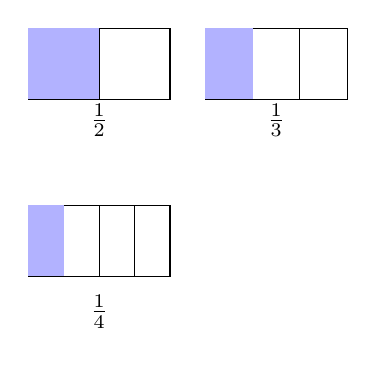
\begin{tikzpicture}[scale=0.9]
\draw (0,0) rectangle (2,1);
\draw (1,0) -- (1,1);
\fill[blue!30] (0,0) rectangle (1,1);
\node at (1,-0.3) {$\frac{1}{2}$};
\draw (2.5,0) rectangle (4.5,1);
\draw (3.17,0) -- (3.17,1);
\draw (3.83,0) -- (3.83,1);
\fill[blue!30] (2.5,0) rectangle (3.17,1);
\node at (3.5,-0.3) {$\frac{1}{3}$};
\draw (0,-2.5) rectangle (2,-1.5);
\draw (0.5,-2.5) -- (0.5,-1.5);
\draw (1,-2.5) -- (1,-1.5);
\draw (1.5,-2.5) -- (1.5,-1.5);
\fill[blue!30] (0,-2.5) rectangle (0.5,-1.5);
\node at (1,-3) {$\frac{1}{4}$};
\end{tikzpicture}
\end{center}

\column{0.55\textwidth}
\textbf{Questions}
\begin{enumerate}
    \item Which is larger: $\frac{1}{2}$ or $\frac{1}{3}$? \ashow{$\frac{1}{2}$}
    \item Compare $\frac{2}{5}$ and $\frac{4}{5}$. Which is bigger? \ashow{$\frac{4}{5}$}
    \item Convert $\frac{3}{4}$ and $\frac{5}{8}$ to a common denominator. Which is larger? \ashow{$\frac{3}{4}=\frac{6}{8}$; larger: $\frac{3}{4}$}
    \item Order from smallest to largest: $\frac{1}{3}, \frac{1}{6}, \frac{1}{2}$. \ashow{$\frac{1}{6},\ \frac{1}{3},\ \frac{1}{2}$}
    \item Sam ate $\frac{2}{3}$ of a pizza, Lee ate $\frac{5}{6}$ of the same pizza. Who ate more? \ashow{Lee ate more.}
    \item Compare $\frac{4}{6}$ and $\frac{2}{3}$. \ashow{Equal: $\frac{4}{6}=\frac{2}{3}$}
\end{enumerate}
\end{columns}

\end{frame}
\begin{frame}<1>{Starter 3: Comparing Fractions}

\begin{columns}
\column{0.45\textwidth}
\begin{center}
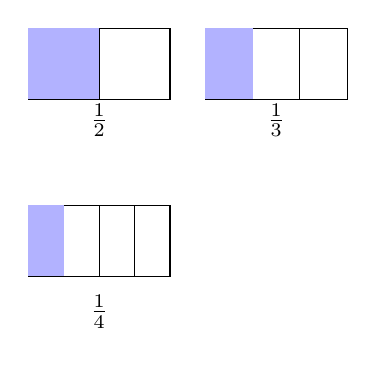
\begin{tikzpicture}[scale=0.9]
\draw (0,0) rectangle (2,1);
\draw (1,0) -- (1,1);
\fill[blue!30] (0,0) rectangle (1,1);
\node at (1,-0.3) {$\frac{1}{2}$};
\draw (2.5,0) rectangle (4.5,1);
\draw (3.17,0) -- (3.17,1);
\draw (3.83,0) -- (3.83,1);
\fill[blue!30] (2.5,0) rectangle (3.17,1);
\node at (3.5,-0.3) {$\frac{1}{3}$};
\draw (0,-2.5) rectangle (2,-1.5);
\draw (0.5,-2.5) -- (0.5,-1.5);
\draw (1,-2.5) -- (1,-1.5);
\draw (1.5,-2.5) -- (1.5,-1.5);
\fill[blue!30] (0,-2.5) rectangle (0.5,-1.5);
\node at (1,-3) {$\frac{1}{4}$};
\end{tikzpicture}
\end{center}

\column{0.55\textwidth}
\textbf{Questions}
\begin{enumerate}
    \item Which is larger: $\frac{1}{2}$ or $\frac{1}{3}$? \ashow{$\frac{1}{2}$}
    \item Compare $\frac{2}{5}$ and $\frac{4}{5}$. Which is bigger? \ashow{$\frac{4}{5}$}
    \item Convert $\frac{3}{4}$ and $\frac{5}{8}$ to a common denominator. Which is larger? \ashow{$\frac{3}{4}=\frac{6}{8}$; larger: $\frac{3}{4}$}
    \item Order from smallest to largest: $\frac{1}{3}, \frac{1}{6}, \frac{1}{2}$. \ashow{$\frac{1}{6},\ \frac{1}{3},\ \frac{1}{2}$}
    \item Sam ate $\frac{2}{3}$ of a pizza, Lee ate $\frac{5}{6}$ of the same pizza. Who ate more? \ashow{Lee ate more.}
    \item Compare $\frac{4}{6}$ and $\frac{2}{3}$. \ashow{Equal: $\frac{4}{6}=\frac{2}{3}$}
\end{enumerate}
\end{columns}

\end{frame}
\begin{frame}<1>{Starter 3: Comparing Fractions}

\begin{columns}
\column{0.45\textwidth}
\begin{center}
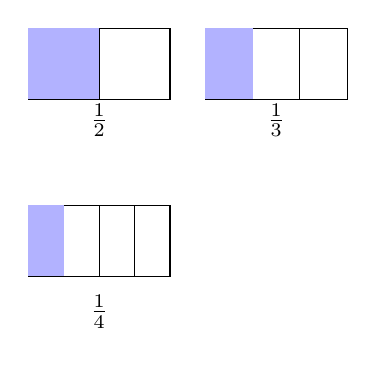
\begin{tikzpicture}[scale=0.9]
\draw (0,0) rectangle (2,1);
\draw (1,0) -- (1,1);
\fill[blue!30] (0,0) rectangle (1,1);
\node at (1,-0.3) {$\frac{1}{2}$};
\draw (2.5,0) rectangle (4.5,1);
\draw (3.17,0) -- (3.17,1);
\draw (3.83,0) -- (3.83,1);
\fill[blue!30] (2.5,0) rectangle (3.17,1);
\node at (3.5,-0.3) {$\frac{1}{3}$};
\draw (0,-2.5) rectangle (2,-1.5);
\draw (0.5,-2.5) -- (0.5,-1.5);
\draw (1,-2.5) -- (1,-1.5);
\draw (1.5,-2.5) -- (1.5,-1.5);
\fill[blue!30] (0,-2.5) rectangle (0.5,-1.5);
\node at (1,-3) {$\frac{1}{4}$};
\end{tikzpicture}
\end{center}

\column{0.55\textwidth}
\textbf{Questions}
\begin{enumerate}
    \item Which is larger: $\frac{1}{2}$ or $\frac{1}{3}$? \ashow{$\frac{1}{2}$}
    \item Compare $\frac{2}{5}$ and $\frac{4}{5}$. Which is bigger? \ashow{$\frac{4}{5}$}
    \item Convert $\frac{3}{4}$ and $\frac{5}{8}$ to a common denominator. Which is larger? \ashow{$\frac{3}{4}=\frac{6}{8}$; larger: $\frac{3}{4}$}
    \item Order from smallest to largest: $\frac{1}{3}, \frac{1}{6}, \frac{1}{2}$. \ashow{$\frac{1}{6},\ \frac{1}{3},\ \frac{1}{2}$}
    \item Sam ate $\frac{2}{3}$ of a pizza, Lee ate $\frac{5}{6}$ of the same pizza. Who ate more? \ashow{Lee ate more.}
    \item Compare $\frac{4}{6}$ and $\frac{2}{3}$. \ashow{Equal: $\frac{4}{6}=\frac{2}{3}$}
\end{enumerate}
\end{columns}

\end{frame}
\begin{frame}<1>{Starter 3: Comparing Fractions}

\begin{columns}
\column{0.45\textwidth}
\begin{center}
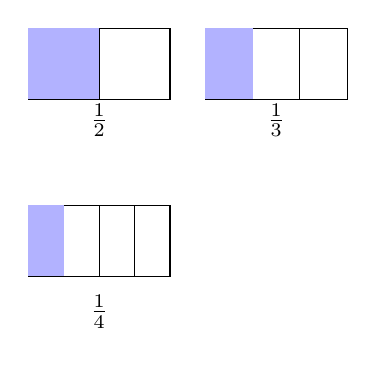
\begin{tikzpicture}[scale=0.9]
\draw (0,0) rectangle (2,1);
\draw (1,0) -- (1,1);
\fill[blue!30] (0,0) rectangle (1,1);
\node at (1,-0.3) {$\frac{1}{2}$};
\draw (2.5,0) rectangle (4.5,1);
\draw (3.17,0) -- (3.17,1);
\draw (3.83,0) -- (3.83,1);
\fill[blue!30] (2.5,0) rectangle (3.17,1);
\node at (3.5,-0.3) {$\frac{1}{3}$};
\draw (0,-2.5) rectangle (2,-1.5);
\draw (0.5,-2.5) -- (0.5,-1.5);
\draw (1,-2.5) -- (1,-1.5);
\draw (1.5,-2.5) -- (1.5,-1.5);
\fill[blue!30] (0,-2.5) rectangle (0.5,-1.5);
\node at (1,-3) {$\frac{1}{4}$};
\end{tikzpicture}
\end{center}

\column{0.55\textwidth}
\textbf{Questions}
\begin{enumerate}
    \item Which is larger: $\frac{1}{2}$ or $\frac{1}{3}$? \ashow{$\frac{1}{2}$}
    \item Compare $\frac{2}{5}$ and $\frac{4}{5}$. Which is bigger? \ashow{$\frac{4}{5}$}
    \item Convert $\frac{3}{4}$ and $\frac{5}{8}$ to a common denominator. Which is larger? \ashow{$\frac{3}{4}=\frac{6}{8}$; larger: $\frac{3}{4}$}
    \item Order from smallest to largest: $\frac{1}{3}, \frac{1}{6}, \frac{1}{2}$. \ashow{$\frac{1}{6},\ \frac{1}{3},\ \frac{1}{2}$}
    \item Sam ate $\frac{2}{3}$ of a pizza, Lee ate $\frac{5}{6}$ of the same pizza. Who ate more? \ashow{Lee ate more.}
    \item Compare $\frac{4}{6}$ and $\frac{2}{3}$. \ashow{Equal: $\frac{4}{6}=\frac{2}{3}$}
\end{enumerate}
\end{columns}

\end{frame}

%------------------------------------------------
% SLIDE 4: Fractions in Real Life
%------------------------------------------------
\begin{frame}<1>{Starter 4}

\begin{columns}
\column{0.45\textwidth}
\begin{center}
\textbf{Fractions everywhere}
\begin{tikzpicture}[scale=0.9]
\draw (0,0) circle (1);
\fill[orange!20] (0,0) -- (0:1) arc (0:90:1) -- cycle;
\fill[orange!20] (0,0) -- (90:1) arc (90:180:1) -- cycle;
\foreach \a in {0,45,90,135,180,225,270,315} {
    \draw (0,0) -- (\a:1);
}

\node at (0,-1.3) {Pizza};
\draw (2,0) rectangle (4,1);
\draw (2.5,0) -- (2.5,1);
\draw (3,0) -- (3,1);
\draw (3.5,0) -- (3.5,1);
\fill[blue!20] (2,0) rectangle (2.5,1);
\node at (3,-0.3) {Chocolate};

% --- Q3 answer: a 24 cm ruler with 1/3 and 1/2 marked ---
\draw[ans] (0,-2.3) rectangle (4,-2.0);
\draw[ans] (1.333,-2.3) -- (1.333,-2.0);
\draw[ans] (2,-2.3) -- (2,-2.0);
\node[anslab, above] at (0.55,-1.97) {$\tfrac{1}{3}=8$ cm};
\node[anslab, above] at (2.65,-1.97) {$\tfrac{1}{2}=12$ cm};
\node[anslab, below right] at (0,-2.35) {0};
\node[anslab, below left] at (4,-2.35) {24 cm};
\end{tikzpicture}
\end{center}

\column{0.55\textwidth}
\textbf{Questions}
\begin{enumerate}
    \item A cake is cut into 10 equal slices. If 3 are eaten, what fraction remains? \ablank{$\frac{7}{10}$}.
    \item There are 30 students. $\frac{2}{5}$ walk to school. How many walk? \ashow{12 students walk}
    \item A ruler is 24 cm long. Mark $\frac{1}{2}$ and $\frac{1}{3}$ on it. How many cm is each?
    \item Which is longer: $\frac{3}{4}$ of an hour or $\frac{2}{3}$ of an hour? (1 hour = 60 mins) \ashow{$\frac{3}{4}$ hour (45 mins) is longer}
    \item You have \$30. You spend $\frac{2}{5}$ on a book. How much do you spend? How much left? \ashow{Spend \$12, left \$18}
    \item A recipe needs $\frac{3}{4}$ cup of milk. You only have a $\frac{1}{4}$ cup measure. How many times must you fill it? \ashow{3 times}
\end{enumerate}
\end{columns}

\end{frame}
\begin{frame}<1>{Starter 4}

\begin{columns}
\column{0.45\textwidth}
\begin{center}
\textbf{Fractions everywhere}
\begin{tikzpicture}[scale=0.9]
\draw (0,0) circle (1);
\fill[orange!20] (0,0) -- (0:1) arc (0:90:1) -- cycle;
\fill[orange!20] (0,0) -- (90:1) arc (90:180:1) -- cycle;
\foreach \a in {0,45,90,135,180,225,270,315} {
    \draw (0,0) -- (\a:1);
}

\node at (0,-1.3) {Pizza};
\draw (2,0) rectangle (4,1);
\draw (2.5,0) -- (2.5,1);
\draw (3,0) -- (3,1);
\draw (3.5,0) -- (3.5,1);
\fill[blue!20] (2,0) rectangle (2.5,1);
\node at (3,-0.3) {Chocolate};

% --- Q3 answer: a 24 cm ruler with 1/3 and 1/2 marked ---
\draw[ans] (0,-2.3) rectangle (4,-2.0);
\draw[ans] (1.333,-2.3) -- (1.333,-2.0);
\draw[ans] (2,-2.3) -- (2,-2.0);
\node[anslab, above] at (0.55,-1.97) {$\tfrac{1}{3}=8$ cm};
\node[anslab, above] at (2.65,-1.97) {$\tfrac{1}{2}=12$ cm};
\node[anslab, below right] at (0,-2.35) {0};
\node[anslab, below left] at (4,-2.35) {24 cm};
\end{tikzpicture}
\end{center}

\column{0.55\textwidth}
\textbf{Questions}
\begin{enumerate}
    \item A cake is cut into 10 equal slices. If 3 are eaten, what fraction remains? \ablank{$\frac{7}{10}$}.
    \item There are 30 students. $\frac{2}{5}$ walk to school. How many walk? \ashow{12 students walk}
    \item A ruler is 24 cm long. Mark $\frac{1}{2}$ and $\frac{1}{3}$ on it. How many cm is each?
    \item Which is longer: $\frac{3}{4}$ of an hour or $\frac{2}{3}$ of an hour? (1 hour = 60 mins) \ashow{$\frac{3}{4}$ hour (45 mins) is longer}
    \item You have \$30. You spend $\frac{2}{5}$ on a book. How much do you spend? How much left? \ashow{Spend \$12, left \$18}
    \item A recipe needs $\frac{3}{4}$ cup of milk. You only have a $\frac{1}{4}$ cup measure. How many times must you fill it? \ashow{3 times}
\end{enumerate}
\end{columns}

\end{frame}
\begin{frame}<1>{Starter 4}

\begin{columns}
\column{0.45\textwidth}
\begin{center}
\textbf{Fractions everywhere}
\begin{tikzpicture}[scale=0.9]
\draw (0,0) circle (1);
\fill[orange!20] (0,0) -- (0:1) arc (0:90:1) -- cycle;
\fill[orange!20] (0,0) -- (90:1) arc (90:180:1) -- cycle;
\foreach \a in {0,45,90,135,180,225,270,315} {
    \draw (0,0) -- (\a:1);
}

\node at (0,-1.3) {Pizza};
\draw (2,0) rectangle (4,1);
\draw (2.5,0) -- (2.5,1);
\draw (3,0) -- (3,1);
\draw (3.5,0) -- (3.5,1);
\fill[blue!20] (2,0) rectangle (2.5,1);
\node at (3,-0.3) {Chocolate};

% --- Q3 answer: a 24 cm ruler with 1/3 and 1/2 marked ---
\draw[ans] (0,-2.3) rectangle (4,-2.0);
\draw[ans] (1.333,-2.3) -- (1.333,-2.0);
\draw[ans] (2,-2.3) -- (2,-2.0);
\node[anslab, above] at (0.55,-1.97) {$\tfrac{1}{3}=8$ cm};
\node[anslab, above] at (2.65,-1.97) {$\tfrac{1}{2}=12$ cm};
\node[anslab, below right] at (0,-2.35) {0};
\node[anslab, below left] at (4,-2.35) {24 cm};
\end{tikzpicture}
\end{center}

\column{0.55\textwidth}
\textbf{Questions}
\begin{enumerate}
    \item A cake is cut into 10 equal slices. If 3 are eaten, what fraction remains? \ablank{$\frac{7}{10}$}.
    \item There are 30 students. $\frac{2}{5}$ walk to school. How many walk? \ashow{12 students walk}
    \item A ruler is 24 cm long. Mark $\frac{1}{2}$ and $\frac{1}{3}$ on it. How many cm is each?
    \item Which is longer: $\frac{3}{4}$ of an hour or $\frac{2}{3}$ of an hour? (1 hour = 60 mins) \ashow{$\frac{3}{4}$ hour (45 mins) is longer}
    \item You have \$30. You spend $\frac{2}{5}$ on a book. How much do you spend? How much left? \ashow{Spend \$12, left \$18}
    \item A recipe needs $\frac{3}{4}$ cup of milk. You only have a $\frac{1}{4}$ cup measure. How many times must you fill it? \ashow{3 times}
\end{enumerate}
\end{columns}

\end{frame}
\begin{frame}<1>{Starter 4}

\begin{columns}
\column{0.45\textwidth}
\begin{center}
\textbf{Fractions everywhere}
\begin{tikzpicture}[scale=0.9]
\draw (0,0) circle (1);
\fill[orange!20] (0,0) -- (0:1) arc (0:90:1) -- cycle;
\fill[orange!20] (0,0) -- (90:1) arc (90:180:1) -- cycle;
\foreach \a in {0,45,90,135,180,225,270,315} {
    \draw (0,0) -- (\a:1);
}

\node at (0,-1.3) {Pizza};
\draw (2,0) rectangle (4,1);
\draw (2.5,0) -- (2.5,1);
\draw (3,0) -- (3,1);
\draw (3.5,0) -- (3.5,1);
\fill[blue!20] (2,0) rectangle (2.5,1);
\node at (3,-0.3) {Chocolate};

% --- Q3 answer: a 24 cm ruler with 1/3 and 1/2 marked ---
\draw[ans] (0,-2.3) rectangle (4,-2.0);
\draw[ans] (1.333,-2.3) -- (1.333,-2.0);
\draw[ans] (2,-2.3) -- (2,-2.0);
\node[anslab, above] at (0.55,-1.97) {$\tfrac{1}{3}=8$ cm};
\node[anslab, above] at (2.65,-1.97) {$\tfrac{1}{2}=12$ cm};
\node[anslab, below right] at (0,-2.35) {0};
\node[anslab, below left] at (4,-2.35) {24 cm};
\end{tikzpicture}
\end{center}

\column{0.55\textwidth}
\textbf{Questions}
\begin{enumerate}
    \item A cake is cut into 10 equal slices. If 3 are eaten, what fraction remains? \ablank{$\frac{7}{10}$}.
    \item There are 30 students. $\frac{2}{5}$ walk to school. How many walk? \ashow{12 students walk}
    \item A ruler is 24 cm long. Mark $\frac{1}{2}$ and $\frac{1}{3}$ on it. How many cm is each?
    \item Which is longer: $\frac{3}{4}$ of an hour or $\frac{2}{3}$ of an hour? (1 hour = 60 mins) \ashow{$\frac{3}{4}$ hour (45 mins) is longer}
    \item You have \$30. You spend $\frac{2}{5}$ on a book. How much do you spend? How much left? \ashow{Spend \$12, left \$18}
    \item A recipe needs $\frac{3}{4}$ cup of milk. You only have a $\frac{1}{4}$ cup measure. How many times must you fill it? \ashow{3 times}
\end{enumerate}
\end{columns}

\end{frame}



\begin{frame}<1>{Starter 5}

\vspace{-3em}

\begin{columns}

% LEFT COLUMN: BARS + A SMALL NUMBER LINE
\column{0.25\textwidth}

\begin{center}
\begin{tikzpicture}[scale=0.9]
% --- Bars for 2/3, 4/6, 6/9 ---
% 2/3 bar
\draw (0,0) rectangle (3,0.6);
\fill[green!35] (0,0) rectangle (2,0.6);

\draw (1,0) -- (1,0.6);
\draw (2,0) -- (2,0.6);

% 4/6 bar
\draw (0,-1.2) rectangle (3,-0.6);
\fill[green!35] (0,-1.2) rectangle (2,-0.6);

\foreach \x in {0.5,1,1.5,2,2.5} \draw (\x,-1.2) -- (\x,-0.6);

% 6/9 bar
\draw (0,-2.4) rectangle (3,-1.8);
\fill[green!35] (0,-2.4) rectangle (2,-1.8);

\foreach \x in {0.333,0.666,1,1.333,1.666,2,2.333,2.666} \draw (\x,-2.4) -- (\x,-1.8);

% --- Compact number line 0 to 3 ---
\draw (-0.1,-3.6) -- (3.1,-3.6);
\foreach \x/\lab in {0/0,1/1,2/2,3/3} {
  \draw (\x,-3.65) -- (\x,-3.55);
  \node at (\x,-3.85) {\small \lab};
}

% --- Q4 answer: the two mixed numbers marked on the number line ---
\fill[ans] (1.667,-3.6) circle (0.06);
\node[anslab, above, inner sep=2pt] at (1.667,-3.55) {$1\tfrac{2}{3}$};
\fill[ans] (2.5,-3.6) circle (0.06);
\node[anslab, above, inner sep=2pt] at (2.5,-3.55) {$2\tfrac{1}{2}$};
\end{tikzpicture}
\end{center}

% RIGHT COLUMN: TWO-COLUMN QUESTIONS (FLOW)
\column{0.75\textwidth}

\small 

\begin{multicols}{2}
\begin{enumerate}
  \item $\dfrac{1}{2}=\dfrac{\ashowq{3}}{6}$
  \item Write the fraction represented by each bar. (Extension) show that they are equivalent \ashow{$\frac{2}{3},\ \frac{4}{6},\ \frac{6}{9}$}
  \item $\dfrac{5}{6}=\dfrac{10}{\ashowq{12}}$


    \item Mark $1\dfrac{2}{3}$ and $2\dfrac{1}{2}$ on the number line. Convert each to an improper fraction. \ashow{$1\frac{2}{3}=\frac{5}{3}$; $2\frac{1}{2}=\frac{5}{2}$}

  \item $\dfrac{2}{3}=\dfrac{\ashowq{8}}{12}$

    \columnbreak

  \item Which are equivalent to $\dfrac{3}{7}$: $\dfrac{9}{21}, \dfrac{6}{14}, \dfrac{12}{28}, \dfrac{8}{21}$? \ashow{$\frac{9}{21},\ \frac{6}{14},\ \frac{12}{28}$}
  \item Write 3 fractions equivalent to $\dfrac{4}{9}$ \ashow{$\frac{8}{18},\ \frac{12}{27},\ \frac{16}{36}$}
  \item Compare ( $<$ $>$ $=$) these fractions: $\dfrac{2}{5}\ \square\ \dfrac{6}{15}$ \ashow{$=$}

  \item Fully simplify $\dfrac{48}{18}$ \ashow{$\frac{8}{3}$ (or $2\frac{2}{3}$)}
\end{enumerate}
\end{multicols}

\end{columns}

\end{frame}
\begin{frame}<1>{Starter 5}

\vspace{-3em}

\begin{columns}

% LEFT COLUMN: BARS + A SMALL NUMBER LINE
\column{0.25\textwidth}

\begin{center}
\begin{tikzpicture}[scale=0.9]
% --- Bars for 2/3, 4/6, 6/9 ---
% 2/3 bar
\draw (0,0) rectangle (3,0.6);
\fill[green!35] (0,0) rectangle (2,0.6);

\draw (1,0) -- (1,0.6);
\draw (2,0) -- (2,0.6);

% 4/6 bar
\draw (0,-1.2) rectangle (3,-0.6);
\fill[green!35] (0,-1.2) rectangle (2,-0.6);

\foreach \x in {0.5,1,1.5,2,2.5} \draw (\x,-1.2) -- (\x,-0.6);

% 6/9 bar
\draw (0,-2.4) rectangle (3,-1.8);
\fill[green!35] (0,-2.4) rectangle (2,-1.8);

\foreach \x in {0.333,0.666,1,1.333,1.666,2,2.333,2.666} \draw (\x,-2.4) -- (\x,-1.8);

% --- Compact number line 0 to 3 ---
\draw (-0.1,-3.6) -- (3.1,-3.6);
\foreach \x/\lab in {0/0,1/1,2/2,3/3} {
  \draw (\x,-3.65) -- (\x,-3.55);
  \node at (\x,-3.85) {\small \lab};
}

% --- Q4 answer: the two mixed numbers marked on the number line ---
\fill[ans] (1.667,-3.6) circle (0.06);
\node[anslab, above, inner sep=2pt] at (1.667,-3.55) {$1\tfrac{2}{3}$};
\fill[ans] (2.5,-3.6) circle (0.06);
\node[anslab, above, inner sep=2pt] at (2.5,-3.55) {$2\tfrac{1}{2}$};
\end{tikzpicture}
\end{center}

% RIGHT COLUMN: TWO-COLUMN QUESTIONS (FLOW)
\column{0.75\textwidth}

\small 

\begin{multicols}{2}
\begin{enumerate}
  \item $\dfrac{1}{2}=\dfrac{\ashowq{3}}{6}$
  \item Write the fraction represented by each bar. (Extension) show that they are equivalent \ashow{$\frac{2}{3},\ \frac{4}{6},\ \frac{6}{9}$}
  \item $\dfrac{5}{6}=\dfrac{10}{\ashowq{12}}$


    \item Mark $1\dfrac{2}{3}$ and $2\dfrac{1}{2}$ on the number line. Convert each to an improper fraction. \ashow{$1\frac{2}{3}=\frac{5}{3}$; $2\frac{1}{2}=\frac{5}{2}$}

  \item $\dfrac{2}{3}=\dfrac{\ashowq{8}}{12}$

    \columnbreak

  \item Which are equivalent to $\dfrac{3}{7}$: $\dfrac{9}{21}, \dfrac{6}{14}, \dfrac{12}{28}, \dfrac{8}{21}$? \ashow{$\frac{9}{21},\ \frac{6}{14},\ \frac{12}{28}$}
  \item Write 3 fractions equivalent to $\dfrac{4}{9}$ \ashow{$\frac{8}{18},\ \frac{12}{27},\ \frac{16}{36}$}
  \item Compare ( $<$ $>$ $=$) these fractions: $\dfrac{2}{5}\ \square\ \dfrac{6}{15}$ \ashow{$=$}

  \item Fully simplify $\dfrac{48}{18}$ \ashow{$\frac{8}{3}$ (or $2\frac{2}{3}$)}
\end{enumerate}
\end{multicols}

\end{columns}

\end{frame}
\begin{frame}<1>{Starter 5}

\vspace{-3em}

\begin{columns}

% LEFT COLUMN: BARS + A SMALL NUMBER LINE
\column{0.25\textwidth}

\begin{center}
\begin{tikzpicture}[scale=0.9]
% --- Bars for 2/3, 4/6, 6/9 ---
% 2/3 bar
\draw (0,0) rectangle (3,0.6);
\fill[green!35] (0,0) rectangle (2,0.6);

\draw (1,0) -- (1,0.6);
\draw (2,0) -- (2,0.6);

% 4/6 bar
\draw (0,-1.2) rectangle (3,-0.6);
\fill[green!35] (0,-1.2) rectangle (2,-0.6);

\foreach \x in {0.5,1,1.5,2,2.5} \draw (\x,-1.2) -- (\x,-0.6);

% 6/9 bar
\draw (0,-2.4) rectangle (3,-1.8);
\fill[green!35] (0,-2.4) rectangle (2,-1.8);

\foreach \x in {0.333,0.666,1,1.333,1.666,2,2.333,2.666} \draw (\x,-2.4) -- (\x,-1.8);

% --- Compact number line 0 to 3 ---
\draw (-0.1,-3.6) -- (3.1,-3.6);
\foreach \x/\lab in {0/0,1/1,2/2,3/3} {
  \draw (\x,-3.65) -- (\x,-3.55);
  \node at (\x,-3.85) {\small \lab};
}

% --- Q4 answer: the two mixed numbers marked on the number line ---
\fill[ans] (1.667,-3.6) circle (0.06);
\node[anslab, above, inner sep=2pt] at (1.667,-3.55) {$1\tfrac{2}{3}$};
\fill[ans] (2.5,-3.6) circle (0.06);
\node[anslab, above, inner sep=2pt] at (2.5,-3.55) {$2\tfrac{1}{2}$};
\end{tikzpicture}
\end{center}

% RIGHT COLUMN: TWO-COLUMN QUESTIONS (FLOW)
\column{0.75\textwidth}

\small 

\begin{multicols}{2}
\begin{enumerate}
  \item $\dfrac{1}{2}=\dfrac{\ashowq{3}}{6}$
  \item Write the fraction represented by each bar. (Extension) show that they are equivalent \ashow{$\frac{2}{3},\ \frac{4}{6},\ \frac{6}{9}$}
  \item $\dfrac{5}{6}=\dfrac{10}{\ashowq{12}}$


    \item Mark $1\dfrac{2}{3}$ and $2\dfrac{1}{2}$ on the number line. Convert each to an improper fraction. \ashow{$1\frac{2}{3}=\frac{5}{3}$; $2\frac{1}{2}=\frac{5}{2}$}

  \item $\dfrac{2}{3}=\dfrac{\ashowq{8}}{12}$

    \columnbreak

  \item Which are equivalent to $\dfrac{3}{7}$: $\dfrac{9}{21}, \dfrac{6}{14}, \dfrac{12}{28}, \dfrac{8}{21}$? \ashow{$\frac{9}{21},\ \frac{6}{14},\ \frac{12}{28}$}
  \item Write 3 fractions equivalent to $\dfrac{4}{9}$ \ashow{$\frac{8}{18},\ \frac{12}{27},\ \frac{16}{36}$}
  \item Compare ( $<$ $>$ $=$) these fractions: $\dfrac{2}{5}\ \square\ \dfrac{6}{15}$ \ashow{$=$}

  \item Fully simplify $\dfrac{48}{18}$ \ashow{$\frac{8}{3}$ (or $2\frac{2}{3}$)}
\end{enumerate}
\end{multicols}

\end{columns}

\end{frame}
\begin{frame}<1>{Starter 5}

\vspace{-3em}

\begin{columns}

% LEFT COLUMN: BARS + A SMALL NUMBER LINE
\column{0.25\textwidth}

\begin{center}
\begin{tikzpicture}[scale=0.9]
% --- Bars for 2/3, 4/6, 6/9 ---
% 2/3 bar
\draw (0,0) rectangle (3,0.6);
\fill[green!35] (0,0) rectangle (2,0.6);

\draw (1,0) -- (1,0.6);
\draw (2,0) -- (2,0.6);

% 4/6 bar
\draw (0,-1.2) rectangle (3,-0.6);
\fill[green!35] (0,-1.2) rectangle (2,-0.6);

\foreach \x in {0.5,1,1.5,2,2.5} \draw (\x,-1.2) -- (\x,-0.6);

% 6/9 bar
\draw (0,-2.4) rectangle (3,-1.8);
\fill[green!35] (0,-2.4) rectangle (2,-1.8);

\foreach \x in {0.333,0.666,1,1.333,1.666,2,2.333,2.666} \draw (\x,-2.4) -- (\x,-1.8);

% --- Compact number line 0 to 3 ---
\draw (-0.1,-3.6) -- (3.1,-3.6);
\foreach \x/\lab in {0/0,1/1,2/2,3/3} {
  \draw (\x,-3.65) -- (\x,-3.55);
  \node at (\x,-3.85) {\small \lab};
}

% --- Q4 answer: the two mixed numbers marked on the number line ---
\fill[ans] (1.667,-3.6) circle (0.06);
\node[anslab, above, inner sep=2pt] at (1.667,-3.55) {$1\tfrac{2}{3}$};
\fill[ans] (2.5,-3.6) circle (0.06);
\node[anslab, above, inner sep=2pt] at (2.5,-3.55) {$2\tfrac{1}{2}$};
\end{tikzpicture}
\end{center}

% RIGHT COLUMN: TWO-COLUMN QUESTIONS (FLOW)
\column{0.75\textwidth}

\small 

\begin{multicols}{2}
\begin{enumerate}
  \item $\dfrac{1}{2}=\dfrac{\ashowq{3}}{6}$
  \item Write the fraction represented by each bar. (Extension) show that they are equivalent \ashow{$\frac{2}{3},\ \frac{4}{6},\ \frac{6}{9}$}
  \item $\dfrac{5}{6}=\dfrac{10}{\ashowq{12}}$


    \item Mark $1\dfrac{2}{3}$ and $2\dfrac{1}{2}$ on the number line. Convert each to an improper fraction. \ashow{$1\frac{2}{3}=\frac{5}{3}$; $2\frac{1}{2}=\frac{5}{2}$}

  \item $\dfrac{2}{3}=\dfrac{\ashowq{8}}{12}$

    \columnbreak

  \item Which are equivalent to $\dfrac{3}{7}$: $\dfrac{9}{21}, \dfrac{6}{14}, \dfrac{12}{28}, \dfrac{8}{21}$? \ashow{$\frac{9}{21},\ \frac{6}{14},\ \frac{12}{28}$}
  \item Write 3 fractions equivalent to $\dfrac{4}{9}$ \ashow{$\frac{8}{18},\ \frac{12}{27},\ \frac{16}{36}$}
  \item Compare ( $<$ $>$ $=$) these fractions: $\dfrac{2}{5}\ \square\ \dfrac{6}{15}$ \ashow{$=$}

  \item Fully simplify $\dfrac{48}{18}$ \ashow{$\frac{8}{3}$ (or $2\frac{2}{3}$)}
\end{enumerate}
\end{multicols}

\end{columns}

\end{frame}


\begin{frame}<1>{Starter 6}

\vspace{-2.5em}

\begin{columns}

% LEFT COLUMN: VISUAL BARS + NUMBER LINE
\column{0.25\textwidth}

\begin{center}
\begin{tikzpicture}[scale=0.9]

% --- Bars for 3/4, 6/8, 9/12 ---
% 3/4
\draw (0,0) rectangle (3,0.6);
\fill[blue!35] (0,0) rectangle (2.25,0.6);
\foreach \x in {0.75,1.5,2.25} \draw (\x,0) -- (\x,0.6);

% 6/8
\draw (0,-1.2) rectangle (3,-0.6);
\fill[blue!35] (0,-1.2) rectangle (2.25,-0.6);
\foreach \x in {0.375,0.75,1.125,1.5,1.875,2.25,2.625} \draw (\x,-1.2) -- (\x,-0.6);

% 9/12
\draw (0,-2.4) rectangle (3,-1.8);
\fill[blue!35] (0,-2.4) rectangle (2.25,-1.8);
\foreach \x in {0.25,0.5,0.75,1,...,2.75} \draw (\x,-2.4) -- (\x,-1.8);

% --- Number Line 0 to 3 ---
\draw (-0.1,-3.6) -- (3.1,-3.6);
\foreach \x/\lab in {0/0,1/1,2/2,3/3} {
  \draw (\x,-3.65) -- (\x,-3.55);
  \node at (\x,-3.85) {\small \lab};
}

% --- Q4 answer: the two mixed numbers marked on the number line ---
\fill[ans] (1.75,-3.6) circle (0.06);
\node[anslab, above, inner sep=2pt] at (1.75,-3.55) {$1\tfrac{3}{4}$};
\fill[ans] (2.667,-3.6) circle (0.06);
\node[anslab, above, inner sep=2pt] at (2.667,-3.55) {$2\tfrac{2}{3}$};
\end{tikzpicture}
\end{center}

% RIGHT COLUMN: QUESTIONS
\column{0.75\textwidth}

\small

\begin{multicols}{2}

\begin{enumerate}

  \item $\dfrac{3}{5}=\dfrac{\ashowq{12}}{20}$

  \item Write the fraction shown by each bar. (Extension) Explain why they represent the same amount. \ashow{$\frac{3}{4},\ \frac{6}{8},\ \frac{9}{12}$}

  \item $\dfrac{4}{7}=\dfrac{\ashowq{12}}{21}$

  \item Mark $1\dfrac{3}{4}$ and $2\dfrac{2}{3}$ on the number line. Convert both to improper fractions. \ashow{$1\frac{3}{4}=\frac{7}{4}$; $2\frac{2}{3}=\frac{8}{3}$}

  \item Fully simplify: $\dfrac{42}{56}$ \ashow{$\frac{3}{4}$}

  \columnbreak

  \item Which are equivalent to $\dfrac{5}{9}$:  
    $\dfrac{10}{18},\ \dfrac{15}{27},\ \dfrac{12}{20},\ \dfrac{25}{45}$? \ashow{$\frac{10}{18},\ \frac{15}{27},\ \frac{25}{45}$}

  \item Write 3 fractions equivalent to $\dfrac{7}{12}$. \ashow{$\frac{14}{24},\ \frac{21}{36},\ \frac{28}{48}$}

  \item Order these fractions in ascending order:  
  \[
  \frac{2}{8},\quad \frac{4}{6},\quad \frac{5}{12}
  \]
  \ashow{$\frac{2}{8},\ \frac{5}{12},\ \frac{4}{6}$}

  \item Compare using $<$, $>$, or $=$:  
  \[
  \frac{9}{14}\ \square\ \frac{19}{28}
  \]
  \ashow{$<$}

\end{enumerate}

\end{multicols}

\end{columns}

\end{frame}
\begin{frame}<1>{Starter 6}

\vspace{-2.5em}

\begin{columns}

% LEFT COLUMN: VISUAL BARS + NUMBER LINE
\column{0.25\textwidth}

\begin{center}
\begin{tikzpicture}[scale=0.9]

% --- Bars for 3/4, 6/8, 9/12 ---
% 3/4
\draw (0,0) rectangle (3,0.6);
\fill[blue!35] (0,0) rectangle (2.25,0.6);
\foreach \x in {0.75,1.5,2.25} \draw (\x,0) -- (\x,0.6);

% 6/8
\draw (0,-1.2) rectangle (3,-0.6);
\fill[blue!35] (0,-1.2) rectangle (2.25,-0.6);
\foreach \x in {0.375,0.75,1.125,1.5,1.875,2.25,2.625} \draw (\x,-1.2) -- (\x,-0.6);

% 9/12
\draw (0,-2.4) rectangle (3,-1.8);
\fill[blue!35] (0,-2.4) rectangle (2.25,-1.8);
\foreach \x in {0.25,0.5,0.75,1,...,2.75} \draw (\x,-2.4) -- (\x,-1.8);

% --- Number Line 0 to 3 ---
\draw (-0.1,-3.6) -- (3.1,-3.6);
\foreach \x/\lab in {0/0,1/1,2/2,3/3} {
  \draw (\x,-3.65) -- (\x,-3.55);
  \node at (\x,-3.85) {\small \lab};
}

% --- Q4 answer: the two mixed numbers marked on the number line ---
\fill[ans] (1.75,-3.6) circle (0.06);
\node[anslab, above, inner sep=2pt] at (1.75,-3.55) {$1\tfrac{3}{4}$};
\fill[ans] (2.667,-3.6) circle (0.06);
\node[anslab, above, inner sep=2pt] at (2.667,-3.55) {$2\tfrac{2}{3}$};
\end{tikzpicture}
\end{center}

% RIGHT COLUMN: QUESTIONS
\column{0.75\textwidth}

\small

\begin{multicols}{2}

\begin{enumerate}

  \item $\dfrac{3}{5}=\dfrac{\ashowq{12}}{20}$

  \item Write the fraction shown by each bar. (Extension) Explain why they represent the same amount. \ashow{$\frac{3}{4},\ \frac{6}{8},\ \frac{9}{12}$}

  \item $\dfrac{4}{7}=\dfrac{\ashowq{12}}{21}$

  \item Mark $1\dfrac{3}{4}$ and $2\dfrac{2}{3}$ on the number line. Convert both to improper fractions. \ashow{$1\frac{3}{4}=\frac{7}{4}$; $2\frac{2}{3}=\frac{8}{3}$}

  \item Fully simplify: $\dfrac{42}{56}$ \ashow{$\frac{3}{4}$}

  \columnbreak

  \item Which are equivalent to $\dfrac{5}{9}$:  
    $\dfrac{10}{18},\ \dfrac{15}{27},\ \dfrac{12}{20},\ \dfrac{25}{45}$? \ashow{$\frac{10}{18},\ \frac{15}{27},\ \frac{25}{45}$}

  \item Write 3 fractions equivalent to $\dfrac{7}{12}$. \ashow{$\frac{14}{24},\ \frac{21}{36},\ \frac{28}{48}$}

  \item Order these fractions in ascending order:  
  \[
  \frac{2}{8},\quad \frac{4}{6},\quad \frac{5}{12}
  \]
  \ashow{$\frac{2}{8},\ \frac{5}{12},\ \frac{4}{6}$}

  \item Compare using $<$, $>$, or $=$:  
  \[
  \frac{9}{14}\ \square\ \frac{19}{28}
  \]
  \ashow{$<$}

\end{enumerate}

\end{multicols}

\end{columns}

\end{frame}
\begin{frame}<1>{Starter 6}

\vspace{-2.5em}

\begin{columns}

% LEFT COLUMN: VISUAL BARS + NUMBER LINE
\column{0.25\textwidth}

\begin{center}
\begin{tikzpicture}[scale=0.9]

% --- Bars for 3/4, 6/8, 9/12 ---
% 3/4
\draw (0,0) rectangle (3,0.6);
\fill[blue!35] (0,0) rectangle (2.25,0.6);
\foreach \x in {0.75,1.5,2.25} \draw (\x,0) -- (\x,0.6);

% 6/8
\draw (0,-1.2) rectangle (3,-0.6);
\fill[blue!35] (0,-1.2) rectangle (2.25,-0.6);
\foreach \x in {0.375,0.75,1.125,1.5,1.875,2.25,2.625} \draw (\x,-1.2) -- (\x,-0.6);

% 9/12
\draw (0,-2.4) rectangle (3,-1.8);
\fill[blue!35] (0,-2.4) rectangle (2.25,-1.8);
\foreach \x in {0.25,0.5,0.75,1,...,2.75} \draw (\x,-2.4) -- (\x,-1.8);

% --- Number Line 0 to 3 ---
\draw (-0.1,-3.6) -- (3.1,-3.6);
\foreach \x/\lab in {0/0,1/1,2/2,3/3} {
  \draw (\x,-3.65) -- (\x,-3.55);
  \node at (\x,-3.85) {\small \lab};
}

% --- Q4 answer: the two mixed numbers marked on the number line ---
\fill[ans] (1.75,-3.6) circle (0.06);
\node[anslab, above, inner sep=2pt] at (1.75,-3.55) {$1\tfrac{3}{4}$};
\fill[ans] (2.667,-3.6) circle (0.06);
\node[anslab, above, inner sep=2pt] at (2.667,-3.55) {$2\tfrac{2}{3}$};
\end{tikzpicture}
\end{center}

% RIGHT COLUMN: QUESTIONS
\column{0.75\textwidth}

\small

\begin{multicols}{2}

\begin{enumerate}

  \item $\dfrac{3}{5}=\dfrac{\ashowq{12}}{20}$

  \item Write the fraction shown by each bar. (Extension) Explain why they represent the same amount. \ashow{$\frac{3}{4},\ \frac{6}{8},\ \frac{9}{12}$}

  \item $\dfrac{4}{7}=\dfrac{\ashowq{12}}{21}$

  \item Mark $1\dfrac{3}{4}$ and $2\dfrac{2}{3}$ on the number line. Convert both to improper fractions. \ashow{$1\frac{3}{4}=\frac{7}{4}$; $2\frac{2}{3}=\frac{8}{3}$}

  \item Fully simplify: $\dfrac{42}{56}$ \ashow{$\frac{3}{4}$}

  \columnbreak

  \item Which are equivalent to $\dfrac{5}{9}$:  
    $\dfrac{10}{18},\ \dfrac{15}{27},\ \dfrac{12}{20},\ \dfrac{25}{45}$? \ashow{$\frac{10}{18},\ \frac{15}{27},\ \frac{25}{45}$}

  \item Write 3 fractions equivalent to $\dfrac{7}{12}$. \ashow{$\frac{14}{24},\ \frac{21}{36},\ \frac{28}{48}$}

  \item Order these fractions in ascending order:  
  \[
  \frac{2}{8},\quad \frac{4}{6},\quad \frac{5}{12}
  \]
  \ashow{$\frac{2}{8},\ \frac{5}{12},\ \frac{4}{6}$}

  \item Compare using $<$, $>$, or $=$:  
  \[
  \frac{9}{14}\ \square\ \frac{19}{28}
  \]
  \ashow{$<$}

\end{enumerate}

\end{multicols}

\end{columns}

\end{frame}
\begin{frame}<1>{Starter 6}

\vspace{-2.5em}

\begin{columns}

% LEFT COLUMN: VISUAL BARS + NUMBER LINE
\column{0.25\textwidth}

\begin{center}
\begin{tikzpicture}[scale=0.9]

% --- Bars for 3/4, 6/8, 9/12 ---
% 3/4
\draw (0,0) rectangle (3,0.6);
\fill[blue!35] (0,0) rectangle (2.25,0.6);
\foreach \x in {0.75,1.5,2.25} \draw (\x,0) -- (\x,0.6);

% 6/8
\draw (0,-1.2) rectangle (3,-0.6);
\fill[blue!35] (0,-1.2) rectangle (2.25,-0.6);
\foreach \x in {0.375,0.75,1.125,1.5,1.875,2.25,2.625} \draw (\x,-1.2) -- (\x,-0.6);

% 9/12
\draw (0,-2.4) rectangle (3,-1.8);
\fill[blue!35] (0,-2.4) rectangle (2.25,-1.8);
\foreach \x in {0.25,0.5,0.75,1,...,2.75} \draw (\x,-2.4) -- (\x,-1.8);

% --- Number Line 0 to 3 ---
\draw (-0.1,-3.6) -- (3.1,-3.6);
\foreach \x/\lab in {0/0,1/1,2/2,3/3} {
  \draw (\x,-3.65) -- (\x,-3.55);
  \node at (\x,-3.85) {\small \lab};
}

% --- Q4 answer: the two mixed numbers marked on the number line ---
\fill[ans] (1.75,-3.6) circle (0.06);
\node[anslab, above, inner sep=2pt] at (1.75,-3.55) {$1\tfrac{3}{4}$};
\fill[ans] (2.667,-3.6) circle (0.06);
\node[anslab, above, inner sep=2pt] at (2.667,-3.55) {$2\tfrac{2}{3}$};
\end{tikzpicture}
\end{center}

% RIGHT COLUMN: QUESTIONS
\column{0.75\textwidth}

\small

\begin{multicols}{2}

\begin{enumerate}

  \item $\dfrac{3}{5}=\dfrac{\ashowq{12}}{20}$

  \item Write the fraction shown by each bar. (Extension) Explain why they represent the same amount. \ashow{$\frac{3}{4},\ \frac{6}{8},\ \frac{9}{12}$}

  \item $\dfrac{4}{7}=\dfrac{\ashowq{12}}{21}$

  \item Mark $1\dfrac{3}{4}$ and $2\dfrac{2}{3}$ on the number line. Convert both to improper fractions. \ashow{$1\frac{3}{4}=\frac{7}{4}$; $2\frac{2}{3}=\frac{8}{3}$}

  \item Fully simplify: $\dfrac{42}{56}$ \ashow{$\frac{3}{4}$}

  \columnbreak

  \item Which are equivalent to $\dfrac{5}{9}$:  
    $\dfrac{10}{18},\ \dfrac{15}{27},\ \dfrac{12}{20},\ \dfrac{25}{45}$? \ashow{$\frac{10}{18},\ \frac{15}{27},\ \frac{25}{45}$}

  \item Write 3 fractions equivalent to $\dfrac{7}{12}$. \ashow{$\frac{14}{24},\ \frac{21}{36},\ \frac{28}{48}$}

  \item Order these fractions in ascending order:  
  \[
  \frac{2}{8},\quad \frac{4}{6},\quad \frac{5}{12}
  \]
  \ashow{$\frac{2}{8},\ \frac{5}{12},\ \frac{4}{6}$}

  \item Compare using $<$, $>$, or $=$:  
  \[
  \frac{9}{14}\ \square\ \frac{19}{28}
  \]
  \ashow{$<$}

\end{enumerate}

\end{multicols}

\end{columns}

\end{frame}


%------------------------------------------------
% SLIDE 7: Same Numerator Comparisons + Simplifying
%------------------------------------------------
\begin{frame}<1>{Starter 7}

\vspace{-2.5em}

\begin{columns}

\column{0.25\textwidth}

\begin{center}
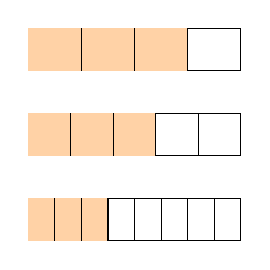
\begin{tikzpicture}[scale=0.9]

% 3/4
\draw (0,0) rectangle (3,0.6);
\fill[orange!35] (0,0) rectangle (2.25,0.6);
\foreach \x in {0.75,1.5,2.25} \draw (\x,0) -- (\x,0.6);

% 3/5
\draw (0,-1.2) rectangle (3,-0.6);
\fill[orange!35] (0,-1.2) rectangle (1.8,-0.6);
\foreach \x in {0.6,1.2,1.8,2.4} \draw (\x,-1.2) -- (\x,-0.6);

% 3/8
\draw (0,-2.4) rectangle (3,-1.8);
\fill[orange!35] (0,-2.4) rectangle (1.125,-1.8);
\foreach \x in {0.375,0.75,1.125,1.5,1.875,2.25,2.625} \draw (\x,-2.4) -- (\x,-1.8);

\end{tikzpicture}
\end{center}

\column{0.75\textwidth}

\small
\begin{multicols}{2}

\begin{enumerate}

\item Write the fraction represented by each bar. \ashow{$\frac{3}{4},\ \frac{3}{5},\ \frac{3}{8}$}

\item Which is largest:  
\[
\frac{3}{4},\quad \frac{3}{5},\quad \frac{3}{8}
\]
\ashow{$\frac{3}{4}$}

\item (Extension) explain why fractions with the same numerator change size when the denominator changes. \ashow{The larger the denominator, the smaller each equal part is.}

\item Compare using $<$, $>$ or $=$:

\[
\frac{5}{6}\ \square\ \frac{5}{9}
\]
\ashow{$>$}

\item Fully simplify: $\frac{18}{24}$ \ashow{$\frac{3}{4}$}

\columnbreak

\item Fully simplify: $
\frac{27}{36}
$ \ashow{$\frac{3}{4}$}

\item Write these as mixed numbers:

\[
\frac{11}{4},\quad \frac{9}{2}
\]
\ashow{$2\frac{3}{4},\ 4\frac{1}{2}$}

\item Convert to improper fractions:

\[
2\frac{3}{5},\quad 1\frac{7}{8}
\]
\ashow{$\frac{13}{5},\ \frac{15}{8}$}

\item Which is bigger:

\[
\frac{7}{10}\ \square\ \frac{7}{12}
\]
\ashow{$\frac{7}{10}$}

\end{enumerate}

\end{multicols}

\end{columns}

\end{frame}
\begin{frame}<1>{Starter 7}

\vspace{-2.5em}

\begin{columns}

\column{0.25\textwidth}

\begin{center}
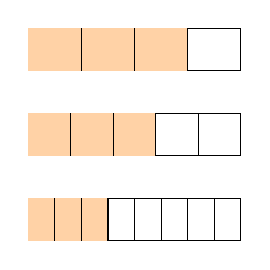
\begin{tikzpicture}[scale=0.9]

% 3/4
\draw (0,0) rectangle (3,0.6);
\fill[orange!35] (0,0) rectangle (2.25,0.6);
\foreach \x in {0.75,1.5,2.25} \draw (\x,0) -- (\x,0.6);

% 3/5
\draw (0,-1.2) rectangle (3,-0.6);
\fill[orange!35] (0,-1.2) rectangle (1.8,-0.6);
\foreach \x in {0.6,1.2,1.8,2.4} \draw (\x,-1.2) -- (\x,-0.6);

% 3/8
\draw (0,-2.4) rectangle (3,-1.8);
\fill[orange!35] (0,-2.4) rectangle (1.125,-1.8);
\foreach \x in {0.375,0.75,1.125,1.5,1.875,2.25,2.625} \draw (\x,-2.4) -- (\x,-1.8);

\end{tikzpicture}
\end{center}

\column{0.75\textwidth}

\small
\begin{multicols}{2}

\begin{enumerate}

\item Write the fraction represented by each bar. \ashow{$\frac{3}{4},\ \frac{3}{5},\ \frac{3}{8}$}

\item Which is largest:  
\[
\frac{3}{4},\quad \frac{3}{5},\quad \frac{3}{8}
\]
\ashow{$\frac{3}{4}$}

\item (Extension) explain why fractions with the same numerator change size when the denominator changes. \ashow{The larger the denominator, the smaller each equal part is.}

\item Compare using $<$, $>$ or $=$:

\[
\frac{5}{6}\ \square\ \frac{5}{9}
\]
\ashow{$>$}

\item Fully simplify: $\frac{18}{24}$ \ashow{$\frac{3}{4}$}

\columnbreak

\item Fully simplify: $
\frac{27}{36}
$ \ashow{$\frac{3}{4}$}

\item Write these as mixed numbers:

\[
\frac{11}{4},\quad \frac{9}{2}
\]
\ashow{$2\frac{3}{4},\ 4\frac{1}{2}$}

\item Convert to improper fractions:

\[
2\frac{3}{5},\quad 1\frac{7}{8}
\]
\ashow{$\frac{13}{5},\ \frac{15}{8}$}

\item Which is bigger:

\[
\frac{7}{10}\ \square\ \frac{7}{12}
\]
\ashow{$\frac{7}{10}$}

\end{enumerate}

\end{multicols}

\end{columns}

\end{frame}
\begin{frame}<1>{Starter 7}

\vspace{-2.5em}

\begin{columns}

\column{0.25\textwidth}

\begin{center}
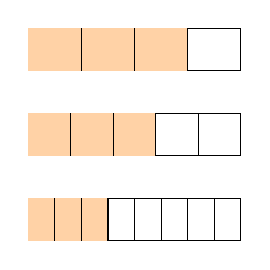
\begin{tikzpicture}[scale=0.9]

% 3/4
\draw (0,0) rectangle (3,0.6);
\fill[orange!35] (0,0) rectangle (2.25,0.6);
\foreach \x in {0.75,1.5,2.25} \draw (\x,0) -- (\x,0.6);

% 3/5
\draw (0,-1.2) rectangle (3,-0.6);
\fill[orange!35] (0,-1.2) rectangle (1.8,-0.6);
\foreach \x in {0.6,1.2,1.8,2.4} \draw (\x,-1.2) -- (\x,-0.6);

% 3/8
\draw (0,-2.4) rectangle (3,-1.8);
\fill[orange!35] (0,-2.4) rectangle (1.125,-1.8);
\foreach \x in {0.375,0.75,1.125,1.5,1.875,2.25,2.625} \draw (\x,-2.4) -- (\x,-1.8);

\end{tikzpicture}
\end{center}

\column{0.75\textwidth}

\small
\begin{multicols}{2}

\begin{enumerate}

\item Write the fraction represented by each bar. \ashow{$\frac{3}{4},\ \frac{3}{5},\ \frac{3}{8}$}

\item Which is largest:  
\[
\frac{3}{4},\quad \frac{3}{5},\quad \frac{3}{8}
\]
\ashow{$\frac{3}{4}$}

\item (Extension) explain why fractions with the same numerator change size when the denominator changes. \ashow{The larger the denominator, the smaller each equal part is.}

\item Compare using $<$, $>$ or $=$:

\[
\frac{5}{6}\ \square\ \frac{5}{9}
\]
\ashow{$>$}

\item Fully simplify: $\frac{18}{24}$ \ashow{$\frac{3}{4}$}

\columnbreak

\item Fully simplify: $
\frac{27}{36}
$ \ashow{$\frac{3}{4}$}

\item Write these as mixed numbers:

\[
\frac{11}{4},\quad \frac{9}{2}
\]
\ashow{$2\frac{3}{4},\ 4\frac{1}{2}$}

\item Convert to improper fractions:

\[
2\frac{3}{5},\quad 1\frac{7}{8}
\]
\ashow{$\frac{13}{5},\ \frac{15}{8}$}

\item Which is bigger:

\[
\frac{7}{10}\ \square\ \frac{7}{12}
\]
\ashow{$\frac{7}{10}$}

\end{enumerate}

\end{multicols}

\end{columns}

\end{frame}
\begin{frame}<1>{Starter 7}

\vspace{-2.5em}

\begin{columns}

\column{0.25\textwidth}

\begin{center}
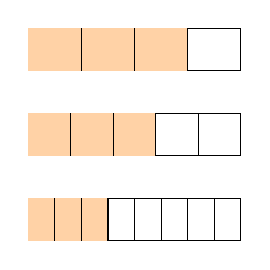
\begin{tikzpicture}[scale=0.9]

% 3/4
\draw (0,0) rectangle (3,0.6);
\fill[orange!35] (0,0) rectangle (2.25,0.6);
\foreach \x in {0.75,1.5,2.25} \draw (\x,0) -- (\x,0.6);

% 3/5
\draw (0,-1.2) rectangle (3,-0.6);
\fill[orange!35] (0,-1.2) rectangle (1.8,-0.6);
\foreach \x in {0.6,1.2,1.8,2.4} \draw (\x,-1.2) -- (\x,-0.6);

% 3/8
\draw (0,-2.4) rectangle (3,-1.8);
\fill[orange!35] (0,-2.4) rectangle (1.125,-1.8);
\foreach \x in {0.375,0.75,1.125,1.5,1.875,2.25,2.625} \draw (\x,-2.4) -- (\x,-1.8);

\end{tikzpicture}
\end{center}

\column{0.75\textwidth}

\small
\begin{multicols}{2}

\begin{enumerate}

\item Write the fraction represented by each bar. \ashow{$\frac{3}{4},\ \frac{3}{5},\ \frac{3}{8}$}

\item Which is largest:  
\[
\frac{3}{4},\quad \frac{3}{5},\quad \frac{3}{8}
\]
\ashow{$\frac{3}{4}$}

\item (Extension) explain why fractions with the same numerator change size when the denominator changes. \ashow{The larger the denominator, the smaller each equal part is.}

\item Compare using $<$, $>$ or $=$:

\[
\frac{5}{6}\ \square\ \frac{5}{9}
\]
\ashow{$>$}

\item Fully simplify: $\frac{18}{24}$ \ashow{$\frac{3}{4}$}

\columnbreak

\item Fully simplify: $
\frac{27}{36}
$ \ashow{$\frac{3}{4}$}

\item Write these as mixed numbers:

\[
\frac{11}{4},\quad \frac{9}{2}
\]
\ashow{$2\frac{3}{4},\ 4\frac{1}{2}$}

\item Convert to improper fractions:

\[
2\frac{3}{5},\quad 1\frac{7}{8}
\]
\ashow{$\frac{13}{5},\ \frac{15}{8}$}

\item Which is bigger:

\[
\frac{7}{10}\ \square\ \frac{7}{12}
\]
\ashow{$\frac{7}{10}$}

\end{enumerate}

\end{multicols}

\end{columns}

\end{frame}



%------------------------------------------------
% SLIDE 8: Diagrams + Mixed Numbers
%------------------------------------------------
\begin{frame}<1>{Starter 8}

\vspace{-2.5em}

\begin{columns}

\column{0.25\textwidth}

\begin{center}
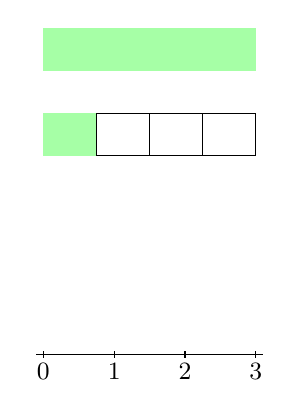
\begin{tikzpicture}[scale=0.9]

% Improper fraction visual (7/4)
\foreach \y in {0,-1.2} {
\draw (0,\y) rectangle (3,\y+0.6);
\foreach \x in {0.75,1.5,2.25} \draw (\x,\y) -- (\x,\y+0.6);
}

\fill[green!35] (0,0) rectangle (3,0.6);
\fill[green!35] (0,-1.2) rectangle (0.75,-0.6);

% number line
\draw (-0.1,-4.0) -- (3.1,-4.0);

\foreach \x/\lab in {0/0,1/1,2/2,3/3} {
\draw (\x,-4.05) -- (\x,-3.95);
\node at (\x,-4.25) {\small \lab};
}

\end{tikzpicture}
\end{center}

\column{0.75\textwidth}

\small
\begin{multicols}{2}

\begin{enumerate}

\item Write the improper fraction shown by the diagram. \ashow{$\frac{5}{4}$}

\item Write the mixed number represented by the green bars in the diagram. \ashow{$1\frac{1}{4}$}

\item Mark $1\frac{1}{4}$ and $2\frac{3}{4}$ on the number line. \ashow{At $1\frac{1}{4}$ and $2\frac{3}{4}$}

\item Convert: $\frac{13}{5}$ to a mixed number. \ashow{$2\frac{3}{5}$}


\item Convert:
\[
3\frac{2}{3}
\]
to an improper fraction. \ashow{$\frac{11}{3}$}

\columnbreak

\item Fully simplify:

\[
\frac{16}{40}
\]
\ashow{$\frac{2}{5}$}

\item Which is greater:

\[
\frac{4}{9}\ \square\ \frac{4}{11}
\]
\ashow{$\frac{4}{9}$}

\item Order from smallest to largest:

\[
\frac{6}{5},\quad 1\frac{1}{2},\quad \frac{7}{4}
\]
\ashow{$\frac{6}{5},\ 1\frac{1}{2},\ \frac{7}{4}$}

\end{enumerate}

\end{multicols}

\end{columns}

\end{frame}
\begin{frame}<1>{Starter 8}

\vspace{-2.5em}

\begin{columns}

\column{0.25\textwidth}

\begin{center}
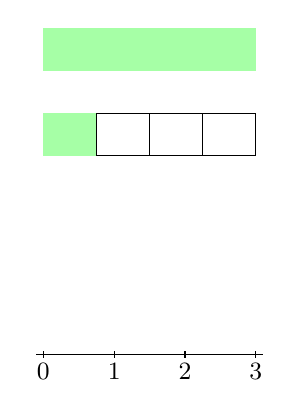
\begin{tikzpicture}[scale=0.9]

% Improper fraction visual (7/4)
\foreach \y in {0,-1.2} {
\draw (0,\y) rectangle (3,\y+0.6);
\foreach \x in {0.75,1.5,2.25} \draw (\x,\y) -- (\x,\y+0.6);
}

\fill[green!35] (0,0) rectangle (3,0.6);
\fill[green!35] (0,-1.2) rectangle (0.75,-0.6);

% number line
\draw (-0.1,-4.0) -- (3.1,-4.0);

\foreach \x/\lab in {0/0,1/1,2/2,3/3} {
\draw (\x,-4.05) -- (\x,-3.95);
\node at (\x,-4.25) {\small \lab};
}

\end{tikzpicture}
\end{center}

\column{0.75\textwidth}

\small
\begin{multicols}{2}

\begin{enumerate}

\item Write the improper fraction shown by the diagram. \ashow{$\frac{5}{4}$}

\item Write the mixed number represented by the green bars in the diagram. \ashow{$1\frac{1}{4}$}

\item Mark $1\frac{1}{4}$ and $2\frac{3}{4}$ on the number line. \ashow{At $1\frac{1}{4}$ and $2\frac{3}{4}$}

\item Convert: $\frac{13}{5}$ to a mixed number. \ashow{$2\frac{3}{5}$}


\item Convert:
\[
3\frac{2}{3}
\]
to an improper fraction. \ashow{$\frac{11}{3}$}

\columnbreak

\item Fully simplify:

\[
\frac{16}{40}
\]
\ashow{$\frac{2}{5}$}

\item Which is greater:

\[
\frac{4}{9}\ \square\ \frac{4}{11}
\]
\ashow{$\frac{4}{9}$}

\item Order from smallest to largest:

\[
\frac{6}{5},\quad 1\frac{1}{2},\quad \frac{7}{4}
\]
\ashow{$\frac{6}{5},\ 1\frac{1}{2},\ \frac{7}{4}$}

\end{enumerate}

\end{multicols}

\end{columns}

\end{frame}
\begin{frame}<1>{Starter 8}

\vspace{-2.5em}

\begin{columns}

\column{0.25\textwidth}

\begin{center}
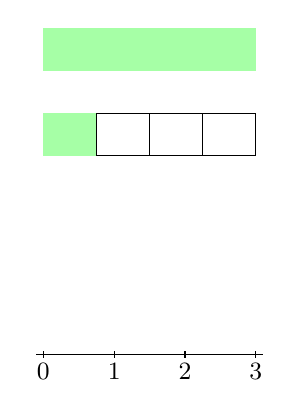
\begin{tikzpicture}[scale=0.9]

% Improper fraction visual (7/4)
\foreach \y in {0,-1.2} {
\draw (0,\y) rectangle (3,\y+0.6);
\foreach \x in {0.75,1.5,2.25} \draw (\x,\y) -- (\x,\y+0.6);
}

\fill[green!35] (0,0) rectangle (3,0.6);
\fill[green!35] (0,-1.2) rectangle (0.75,-0.6);

% number line
\draw (-0.1,-4.0) -- (3.1,-4.0);

\foreach \x/\lab in {0/0,1/1,2/2,3/3} {
\draw (\x,-4.05) -- (\x,-3.95);
\node at (\x,-4.25) {\small \lab};
}

\end{tikzpicture}
\end{center}

\column{0.75\textwidth}

\small
\begin{multicols}{2}

\begin{enumerate}

\item Write the improper fraction shown by the diagram. \ashow{$\frac{5}{4}$}

\item Write the mixed number represented by the green bars in the diagram. \ashow{$1\frac{1}{4}$}

\item Mark $1\frac{1}{4}$ and $2\frac{3}{4}$ on the number line. \ashow{At $1\frac{1}{4}$ and $2\frac{3}{4}$}

\item Convert: $\frac{13}{5}$ to a mixed number. \ashow{$2\frac{3}{5}$}


\item Convert:
\[
3\frac{2}{3}
\]
to an improper fraction. \ashow{$\frac{11}{3}$}

\columnbreak

\item Fully simplify:

\[
\frac{16}{40}
\]
\ashow{$\frac{2}{5}$}

\item Which is greater:

\[
\frac{4}{9}\ \square\ \frac{4}{11}
\]
\ashow{$\frac{4}{9}$}

\item Order from smallest to largest:

\[
\frac{6}{5},\quad 1\frac{1}{2},\quad \frac{7}{4}
\]
\ashow{$\frac{6}{5},\ 1\frac{1}{2},\ \frac{7}{4}$}

\end{enumerate}

\end{multicols}

\end{columns}

\end{frame}
\begin{frame}<1>{Starter 8}

\vspace{-2.5em}

\begin{columns}

\column{0.25\textwidth}

\begin{center}
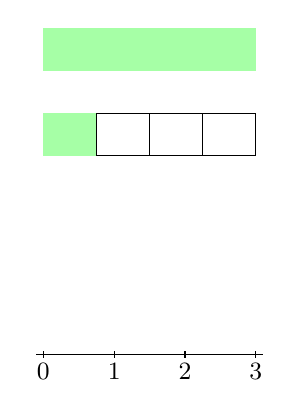
\begin{tikzpicture}[scale=0.9]

% Improper fraction visual (7/4)
\foreach \y in {0,-1.2} {
\draw (0,\y) rectangle (3,\y+0.6);
\foreach \x in {0.75,1.5,2.25} \draw (\x,\y) -- (\x,\y+0.6);
}

\fill[green!35] (0,0) rectangle (3,0.6);
\fill[green!35] (0,-1.2) rectangle (0.75,-0.6);

% number line
\draw (-0.1,-4.0) -- (3.1,-4.0);

\foreach \x/\lab in {0/0,1/1,2/2,3/3} {
\draw (\x,-4.05) -- (\x,-3.95);
\node at (\x,-4.25) {\small \lab};
}

\end{tikzpicture}
\end{center}

\column{0.75\textwidth}

\small
\begin{multicols}{2}

\begin{enumerate}

\item Write the improper fraction shown by the diagram. \ashow{$\frac{5}{4}$}

\item Write the mixed number represented by the green bars in the diagram. \ashow{$1\frac{1}{4}$}

\item Mark $1\frac{1}{4}$ and $2\frac{3}{4}$ on the number line. \ashow{At $1\frac{1}{4}$ and $2\frac{3}{4}$}

\item Convert: $\frac{13}{5}$ to a mixed number. \ashow{$2\frac{3}{5}$}


\item Convert:
\[
3\frac{2}{3}
\]
to an improper fraction. \ashow{$\frac{11}{3}$}

\columnbreak

\item Fully simplify:

\[
\frac{16}{40}
\]
\ashow{$\frac{2}{5}$}

\item Which is greater:

\[
\frac{4}{9}\ \square\ \frac{4}{11}
\]
\ashow{$\frac{4}{9}$}

\item Order from smallest to largest:

\[
\frac{6}{5},\quad 1\frac{1}{2},\quad \frac{7}{4}
\]
\ashow{$\frac{6}{5},\ 1\frac{1}{2},\ \frac{7}{4}$}

\end{enumerate}

\end{multicols}

\end{columns}

\end{frame}



%------------------------------------------------
% SLIDE 9: Review Mix
%------------------------------------------------
\begin{frame}<1>{Starter 9}

\vspace{-2.5em}

\begin{columns}

\column{0.25\textwidth}

\begin{center}
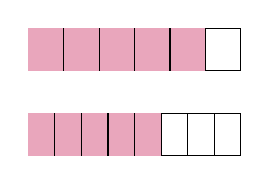
\begin{tikzpicture}[scale=0.9]

% 5/6 bar
\draw (0,0) rectangle (3,0.6);
\fill[purple!35] (0,0) rectangle (2.5,0.6);

\foreach \x in {0.5,1,1.5,2,2.5} \draw (\x,0) -- (\x,0.6);

% 5/8 bar
\draw (0,-1.2) rectangle (3,-0.6);
\fill[purple!35] (0,-1.2) rectangle (1.875,-0.6);

\foreach \x in {0.375,0.75,1.125,1.5,1.875,2.25,2.625} \draw (\x,-1.2) -- (\x,-0.6);

\end{tikzpicture}
\end{center}

\column{0.75\textwidth}

\small
\begin{multicols}{2}

\begin{enumerate}

\item Write the fractions shown by the bars. \ashow{$\frac{5}{6}$ and $\frac{5}{8}$}

\item Which is larger:

\[
\frac{5}{6}\ \square\ \frac{5}{8}
\]
\ashow{$>$}

\item Write 3 fractions equivalent to:

\[
\frac{2}{5}
\]
\ashow{$\frac{4}{10},\ \frac{6}{15},\ \frac{8}{20}$}

\item Fully simplify:
\[
\frac{54}{72}
\]
\ashow{$\frac{3}{4}$}

\item Convert to mixed numbers:

\[
\frac{17}{6},\quad \frac{22}{9}
\]
\ashow{$2\frac{5}{6},\ 2\frac{4}{9}$}

\item Convert to improper fractions:

\[
4\frac{1}{3},\quad 2\frac{5}{6}
\]
\ashow{$\frac{13}{3},\ \frac{17}{6}$}

\item Order from smallest to largest:

\[
\frac{123}{1234},\quad \frac{321}{1234},\quad \frac{111}{1234}
\]
\ashow{$\frac{111}{1234},\ \frac{123}{1234},\ \frac{321}{1234}$}

\item Challenge:

Which is larger?

\[
2\frac{1}{4}\ \square\ 2\frac{2}{5}
\]
\ashow{$2\frac{2}{5}$}

\end{enumerate}

\end{multicols}

\end{columns}

\end{frame}
\begin{frame}<1>{Starter 9}

\vspace{-2.5em}

\begin{columns}

\column{0.25\textwidth}

\begin{center}
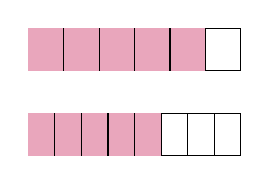
\begin{tikzpicture}[scale=0.9]

% 5/6 bar
\draw (0,0) rectangle (3,0.6);
\fill[purple!35] (0,0) rectangle (2.5,0.6);

\foreach \x in {0.5,1,1.5,2,2.5} \draw (\x,0) -- (\x,0.6);

% 5/8 bar
\draw (0,-1.2) rectangle (3,-0.6);
\fill[purple!35] (0,-1.2) rectangle (1.875,-0.6);

\foreach \x in {0.375,0.75,1.125,1.5,1.875,2.25,2.625} \draw (\x,-1.2) -- (\x,-0.6);

\end{tikzpicture}
\end{center}

\column{0.75\textwidth}

\small
\begin{multicols}{2}

\begin{enumerate}

\item Write the fractions shown by the bars. \ashow{$\frac{5}{6}$ and $\frac{5}{8}$}

\item Which is larger:

\[
\frac{5}{6}\ \square\ \frac{5}{8}
\]
\ashow{$>$}

\item Write 3 fractions equivalent to:

\[
\frac{2}{5}
\]
\ashow{$\frac{4}{10},\ \frac{6}{15},\ \frac{8}{20}$}

\item Fully simplify:
\[
\frac{54}{72}
\]
\ashow{$\frac{3}{4}$}

\item Convert to mixed numbers:

\[
\frac{17}{6},\quad \frac{22}{9}
\]
\ashow{$2\frac{5}{6},\ 2\frac{4}{9}$}

\item Convert to improper fractions:

\[
4\frac{1}{3},\quad 2\frac{5}{6}
\]
\ashow{$\frac{13}{3},\ \frac{17}{6}$}

\item Order from smallest to largest:

\[
\frac{123}{1234},\quad \frac{321}{1234},\quad \frac{111}{1234}
\]
\ashow{$\frac{111}{1234},\ \frac{123}{1234},\ \frac{321}{1234}$}

\item Challenge:

Which is larger?

\[
2\frac{1}{4}\ \square\ 2\frac{2}{5}
\]
\ashow{$2\frac{2}{5}$}

\end{enumerate}

\end{multicols}

\end{columns}

\end{frame}
\begin{frame}<1>{Starter 9}

\vspace{-2.5em}

\begin{columns}

\column{0.25\textwidth}

\begin{center}
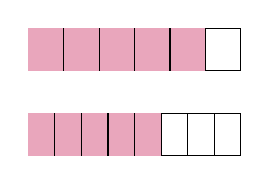
\begin{tikzpicture}[scale=0.9]

% 5/6 bar
\draw (0,0) rectangle (3,0.6);
\fill[purple!35] (0,0) rectangle (2.5,0.6);

\foreach \x in {0.5,1,1.5,2,2.5} \draw (\x,0) -- (\x,0.6);

% 5/8 bar
\draw (0,-1.2) rectangle (3,-0.6);
\fill[purple!35] (0,-1.2) rectangle (1.875,-0.6);

\foreach \x in {0.375,0.75,1.125,1.5,1.875,2.25,2.625} \draw (\x,-1.2) -- (\x,-0.6);

\end{tikzpicture}
\end{center}

\column{0.75\textwidth}

\small
\begin{multicols}{2}

\begin{enumerate}

\item Write the fractions shown by the bars. \ashow{$\frac{5}{6}$ and $\frac{5}{8}$}

\item Which is larger:

\[
\frac{5}{6}\ \square\ \frac{5}{8}
\]
\ashow{$>$}

\item Write 3 fractions equivalent to:

\[
\frac{2}{5}
\]
\ashow{$\frac{4}{10},\ \frac{6}{15},\ \frac{8}{20}$}

\item Fully simplify:
\[
\frac{54}{72}
\]
\ashow{$\frac{3}{4}$}

\item Convert to mixed numbers:

\[
\frac{17}{6},\quad \frac{22}{9}
\]
\ashow{$2\frac{5}{6},\ 2\frac{4}{9}$}

\item Convert to improper fractions:

\[
4\frac{1}{3},\quad 2\frac{5}{6}
\]
\ashow{$\frac{13}{3},\ \frac{17}{6}$}

\item Order from smallest to largest:

\[
\frac{123}{1234},\quad \frac{321}{1234},\quad \frac{111}{1234}
\]
\ashow{$\frac{111}{1234},\ \frac{123}{1234},\ \frac{321}{1234}$}

\item Challenge:

Which is larger?

\[
2\frac{1}{4}\ \square\ 2\frac{2}{5}
\]
\ashow{$2\frac{2}{5}$}

\end{enumerate}

\end{multicols}

\end{columns}

\end{frame}
\begin{frame}<1>{Starter 9}

\vspace{-2.5em}

\begin{columns}

\column{0.25\textwidth}

\begin{center}
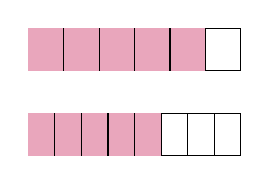
\begin{tikzpicture}[scale=0.9]

% 5/6 bar
\draw (0,0) rectangle (3,0.6);
\fill[purple!35] (0,0) rectangle (2.5,0.6);

\foreach \x in {0.5,1,1.5,2,2.5} \draw (\x,0) -- (\x,0.6);

% 5/8 bar
\draw (0,-1.2) rectangle (3,-0.6);
\fill[purple!35] (0,-1.2) rectangle (1.875,-0.6);

\foreach \x in {0.375,0.75,1.125,1.5,1.875,2.25,2.625} \draw (\x,-1.2) -- (\x,-0.6);

\end{tikzpicture}
\end{center}

\column{0.75\textwidth}

\small
\begin{multicols}{2}

\begin{enumerate}

\item Write the fractions shown by the bars. \ashow{$\frac{5}{6}$ and $\frac{5}{8}$}

\item Which is larger:

\[
\frac{5}{6}\ \square\ \frac{5}{8}
\]
\ashow{$>$}

\item Write 3 fractions equivalent to:

\[
\frac{2}{5}
\]
\ashow{$\frac{4}{10},\ \frac{6}{15},\ \frac{8}{20}$}

\item Fully simplify:
\[
\frac{54}{72}
\]
\ashow{$\frac{3}{4}$}

\item Convert to mixed numbers:

\[
\frac{17}{6},\quad \frac{22}{9}
\]
\ashow{$2\frac{5}{6},\ 2\frac{4}{9}$}

\item Convert to improper fractions:

\[
4\frac{1}{3},\quad 2\frac{5}{6}
\]
\ashow{$\frac{13}{3},\ \frac{17}{6}$}

\item Order from smallest to largest:

\[
\frac{123}{1234},\quad \frac{321}{1234},\quad \frac{111}{1234}
\]
\ashow{$\frac{111}{1234},\ \frac{123}{1234},\ \frac{321}{1234}$}

\item Challenge:

Which is larger?

\[
2\frac{1}{4}\ \square\ 2\frac{2}{5}
\]
\ashow{$2\frac{2}{5}$}

\end{enumerate}

\end{multicols}

\end{columns}

\end{frame}

\end{document}